% This file was converted to LaTeX by Writer2LaTeX ver. 1.0.2
% see http://writer2latex.sourceforge.net for more info
\documentclass[12pt]{article}
\usepackage[utf8]{inputenc}
\usepackage[T1]{fontenc}
\usepackage[english]{babel}
\usepackage{amsmath}
\usepackage{amssymb,amsfonts,textcomp}
\usepackage{array}
\usepackage{supertabular}
\usepackage{hhline}
\usepackage{hyperref}
\hypersetup{colorlinks=true, linkcolor=blue, citecolor=blue, filecolor=blue, urlcolor=blue}
\usepackage{graphicx}
% Text styles
\newcommand\textstyleListLabelxxx[1]{#1}
\makeatletter
\newcommand\arraybslash{\let\\\@arraycr}
\makeatother
\raggedbottom
% Paragraph styles
\renewcommand\familydefault{\rmdefault}
\newenvironment{stylelsSourceline}{\renewcommand\baselinestretch{1.0}\setlength\leftskip{0.748in}\setlength\rightskip{0in plus 1fil}\setlength\parindent{0in}\setlength\parfillskip{0pt plus 1fil}\setlength\parskip{0in plus 1pt}\writerlistparindent\writerlistleftskip\leavevmode\normalfont\normalsize\itshape\writerlistlabel\ignorespaces}{\unskip\vspace{0in plus 1pt}\par}
\newenvironment{stylelsAbstract}{\setlength\leftskip{0.5in}\setlength\rightskip{0.5in}\setlength\parindent{0in}\setlength\parfillskip{0pt plus 1fil}\setlength\parskip{0in plus 1pt}\writerlistparindent\writerlistleftskip\leavevmode\normalfont\normalsize\itshape\writerlistlabel\ignorespaces}{\unskip\vspace{0.111in plus 0.0111in}\par}
\newenvironment{styleStandard}{\setlength\leftskip{0cm}\setlength\rightskip{0cm plus 1fil}\setlength\parindent{0cm}\setlength\parfillskip{0pt plus 1fil}\setlength\parskip{0in plus 1pt}\writerlistparindent\writerlistleftskip\leavevmode\normalfont\normalsize\writerlistlabel\ignorespaces}{\unskip\vspace{0.111in plus 0.0111in}\par}
\newenvironment{stylelsSectioni}{\setlength\leftskip{0.25in}\setlength\rightskip{0in plus 1fil}\setlength\parindent{0in}\setlength\parfillskip{0pt plus 1fil}\setlength\parskip{0.1665in plus 0.016649999in}\writerlistparindent\writerlistleftskip\leavevmode\normalfont\normalsize\fontsize{18pt}{21.6pt}\selectfont\bfseries\writerlistlabel\ignorespaces}{\unskip\vspace{0.0835in plus 0.00835in}\par}
\newenvironment{stylelsSectionii}{\setlength\leftskip{0.25in}\setlength\rightskip{0in plus 1fil}\setlength\parindent{0in}\setlength\parfillskip{0pt plus 1fil}\setlength\parskip{0.222in plus 0.0222in}\writerlistparindent\writerlistleftskip\leavevmode\normalfont\normalsize\fontsize{16pt}{19.2pt}\selectfont\bfseries\writerlistlabel\ignorespaces}{\unskip\vspace{0.0835in plus 0.00835in}\par}
\newenvironment{stylelsEnumerated}{\renewcommand\baselinestretch{1.0}\setlength\leftskip{0cm}\setlength\rightskip{0cm plus 1fil}\setlength\parindent{0cm}\setlength\parfillskip{0pt plus 1fil}\setlength\parskip{0in plus 1pt}\writerlistparindent\writerlistleftskip\leavevmode\normalfont\normalsize\writerlistlabel\ignorespaces}{\unskip\vspace{0.0972in plus 0.00972in}\par}
\newenvironment{stylelsSectioniii}{\setlength\leftskip{0.5717in}\setlength\rightskip{0in plus 1fil}\setlength\parindent{0in}\setlength\parfillskip{0pt plus 1fil}\setlength\parskip{0.0972in plus 0.00972in}\writerlistparindent\writerlistleftskip\leavevmode\normalfont\normalsize\fontsize{14pt}{16.8pt}\selectfont\bfseries\writerlistlabel\ignorespaces}{\unskip\vspace{0in plus 1pt}\par}
\newenvironment{stylelsLanginfo}{\renewcommand\baselinestretch{1.0}\setlength\leftskip{0.0783in}\setlength\rightskip{0in plus 1fil}\setlength\parindent{0in}\setlength\parfillskip{0pt plus 1fil}\setlength\parskip{0in plus 1pt}\writerlistparindent\writerlistleftskip\leavevmode\normalfont\normalsize\writerlistlabel\ignorespaces}{\unskip\vspace{0in plus 1pt}\par}
\newenvironment{styleNormali}{\renewcommand\baselinestretch{1.0}\setlength\leftskip{0cm}\setlength\rightskip{0cm plus 1fil}\setlength\parindent{0cm}\setlength\parfillskip{0pt plus 1fil}\setlength\parskip{0in plus 1pt}\writerlistparindent\writerlistleftskip\leavevmode\normalfont\normalsize\writerlistlabel\ignorespaces}{\unskip\vspace{0.139in plus 0.0139in}\par}
% List styles
\newcommand\writerlistleftskip{}
\newcommand\writerlistparindent{}
\newcommand\writerlistlabel{}
\newcommand\writerlistremovelabel{\aftergroup\let\aftergroup\writerlistparindent\aftergroup\relax\aftergroup\let\aftergroup\writerlistlabel\aftergroup\relax}
\newcounter{listWWNumxxiileveli}
\newcounter{listWWNumxxiilevelii}[listWWNumxxiileveli]
\newcounter{listWWNumxxiileveliii}[listWWNumxxiilevelii]
\newcounter{listWWNumxxiileveliv}[listWWNumxxiileveliii]
\renewcommand\thelistWWNumxxiileveli{\arabic{listWWNumxxiileveli}}
\renewcommand\thelistWWNumxxiilevelii{\arabic{listWWNumxxiileveli}.\arabic{listWWNumxxiilevelii}}
\renewcommand\thelistWWNumxxiileveliii{\arabic{listWWNumxxiileveli}.\arabic{listWWNumxxiilevelii}.\arabic{listWWNumxxiileveliii}}
\renewcommand\thelistWWNumxxiileveliv{\arabic{listWWNumxxiileveli}.\arabic{listWWNumxxiilevelii}.\arabic{listWWNumxxiileveliii}.\arabic{listWWNumxxiileveliv}}
\newcommand\labellistWWNumxxiileveli{\thelistWWNumxxiileveli.}
\newcommand\labellistWWNumxxiilevelii{\thelistWWNumxxiilevelii.}
\newcommand\labellistWWNumxxiileveliii{\thelistWWNumxxiileveliii.}
\newcommand\labellistWWNumxxiileveliv{\thelistWWNumxxiileveliv.}
\newenvironment{listWWNumxxiileveli}{\def\writerlistleftskip{\addtolength\leftskip{0.0cm}}\def\writerlistparindent{}\def\writerlistlabel{}\def\item{\def\writerlistparindent{\setlength\parindent{-0cm}}\def\writerlistlabel{\stepcounter{listWWNumxxiileveli}\makebox[0cm][l]{\labellistWWNumxxiileveli}\hspace{0cm}\writerlistremovelabel}}}{}
\newenvironment{listWWNumxxiilevelii}{\def\writerlistleftskip{\addtolength\leftskip{0.0cm}}\def\writerlistparindent{}\def\writerlistlabel{}\def\item{\def\writerlistparindent{\setlength\parindent{-0cm}}\def\writerlistlabel{\stepcounter{listWWNumxxiilevelii}\makebox[0cm][l]{\labellistWWNumxxiilevelii}\hspace{0cm}\writerlistremovelabel}}}{}
\newenvironment{listWWNumxxiileveliii}{\def\writerlistleftskip{\addtolength\leftskip{0.0cm}}\def\writerlistparindent{}\def\writerlistlabel{}\def\item{\def\writerlistparindent{\setlength\parindent{-0cm}}\def\writerlistlabel{\stepcounter{listWWNumxxiileveliii}\makebox[0cm][r]{\labellistWWNumxxiileveliii}\hspace{0cm}\writerlistremovelabel}}}{}
\newenvironment{listWWNumxxiileveliv}{\def\writerlistleftskip{\addtolength\leftskip{0.0cm}}\def\writerlistparindent{}\def\writerlistlabel{}\def\item{\def\writerlistparindent{\setlength\parindent{-0cm}}\def\writerlistlabel{\stepcounter{listWWNumxxiileveliv}\makebox[0cm][l]{\labellistWWNumxxiileveliv}\hspace{0cm}\writerlistremovelabel}}}{}
\newcounter{listWWNumxleveli}
\newcounter{listWWNumxlevelii}[listWWNumxleveli]
\newcounter{listWWNumxleveliii}[listWWNumxlevelii]
\newcounter{listWWNumxleveliv}[listWWNumxleveliii]
\renewcommand\thelistWWNumxleveli{\arabic{listWWNumxleveli}}
\renewcommand\thelistWWNumxlevelii{\alph{listWWNumxlevelii}}
\renewcommand\thelistWWNumxleveliii{\roman{listWWNumxleveliii}}
\renewcommand\thelistWWNumxleveliv{\arabic{listWWNumxleveliv}}
\newcommand\labellistWWNumxleveli{\thelistWWNumxleveli.}
\newcommand\labellistWWNumxlevelii{\thelistWWNumxlevelii.}
\newcommand\labellistWWNumxleveliii{\thelistWWNumxleveliii.}
\newcommand\labellistWWNumxleveliv{\thelistWWNumxleveliv.}
\newenvironment{listWWNumxleveli}{\def\writerlistleftskip{\addtolength\leftskip{0.0cm}}\def\writerlistparindent{}\def\writerlistlabel{}\def\item{\def\writerlistparindent{\setlength\parindent{-0cm}}\def\writerlistlabel{\stepcounter{listWWNumxleveli}\makebox[0cm][l]{\labellistWWNumxleveli}\hspace{0cm}\writerlistremovelabel}}}{}
\newenvironment{listWWNumxlevelii}{\def\writerlistleftskip{\addtolength\leftskip{0.0cm}}\def\writerlistparindent{}\def\writerlistlabel{}\def\item{\def\writerlistparindent{\setlength\parindent{-0cm}}\def\writerlistlabel{\stepcounter{listWWNumxlevelii}\makebox[0cm][l]{\labellistWWNumxlevelii}\hspace{0cm}\writerlistremovelabel}}}{}
\newenvironment{listWWNumxleveliii}{\def\writerlistleftskip{\addtolength\leftskip{0.0cm}}\def\writerlistparindent{}\def\writerlistlabel{}\def\item{\def\writerlistparindent{\setlength\parindent{-0cm}}\def\writerlistlabel{\stepcounter{listWWNumxleveliii}\makebox[0cm][r]{\labellistWWNumxleveliii}\hspace{0cm}\writerlistremovelabel}}}{}
\newenvironment{listWWNumxleveliv}{\def\writerlistleftskip{\addtolength\leftskip{0.0cm}}\def\writerlistparindent{}\def\writerlistlabel{}\def\item{\def\writerlistparindent{\setlength\parindent{-0cm}}\def\writerlistlabel{\stepcounter{listWWNumxleveliv}\makebox[0cm][l]{\labellistWWNumxleveliv}\hspace{0cm}\writerlistremovelabel}}}{}
\newcounter{listWWNumxxviilevelii}
\newcounter{listWWNumxxviileveliii}[listWWNumxxviilevelii]
\newcounter{listWWNumxxviileveliv}[listWWNumxxviileveliii]
\renewcommand\thelistWWNumxxviilevelii{\alph{listWWNumxxviilevelii}}
\renewcommand\thelistWWNumxxviileveliii{\roman{listWWNumxxviileveliii}}
\renewcommand\thelistWWNumxxviileveliv{\arabic{listWWNumxxviileveliv}}
\newcommand\labellistWWNumxxviileveli{\textstyleListLabelxxx{${\bullet}$}}
\newcommand\labellistWWNumxxviilevelii{\thelistWWNumxxviilevelii)}
\newcommand\labellistWWNumxxviileveliii{\thelistWWNumxxviileveliii)}
\newcommand\labellistWWNumxxviileveliv{(\thelistWWNumxxviileveliv)}
\newenvironment{listWWNumxxviileveli}{\def\writerlistleftskip{\addtolength\leftskip{0.0cm}}\def\writerlistparindent{}\def\writerlistlabel{}\def\item{\def\writerlistparindent{\setlength\parindent{-0cm}}\def\writerlistlabel{\makebox[0cm][l]{\labellistWWNumxxviileveli}\hspace{0cm}\writerlistremovelabel}}}{}
\newenvironment{listWWNumxxviilevelii}{\def\writerlistleftskip{\addtolength\leftskip{0.0cm}}\def\writerlistparindent{}\def\writerlistlabel{}\def\item{\def\writerlistparindent{\setlength\parindent{-0cm}}\def\writerlistlabel{\stepcounter{listWWNumxxviilevelii}\makebox[0cm][l]{\labellistWWNumxxviilevelii}\hspace{0cm}\writerlistremovelabel}}}{}
\newenvironment{listWWNumxxviileveliii}{\def\writerlistleftskip{\addtolength\leftskip{0.0cm}}\def\writerlistparindent{}\def\writerlistlabel{}\def\item{\def\writerlistparindent{\setlength\parindent{-0cm}}\def\writerlistlabel{\stepcounter{listWWNumxxviileveliii}\makebox[0cm][l]{\labellistWWNumxxviileveliii}\hspace{0cm}\writerlistremovelabel}}}{}
\newenvironment{listWWNumxxviileveliv}{\def\writerlistleftskip{\addtolength\leftskip{0.0cm}}\def\writerlistparindent{}\def\writerlistlabel{}\def\item{\def\writerlistparindent{\setlength\parindent{-0cm}}\def\writerlistlabel{\stepcounter{listWWNumxxviileveliv}\makebox[0cm][l]{\labellistWWNumxxviileveliv}\hspace{0cm}\writerlistremovelabel}}}{}
\newcounter{listWWNumiileveli}
\newcounter{listWWNumiilevelii}[listWWNumiileveli]
\newcounter{listWWNumiileveliii}[listWWNumiilevelii]
\newcounter{listWWNumiileveliv}[listWWNumiileveliii]
\renewcommand\thelistWWNumiileveli{\arabic{listWWNumiileveli}}
\renewcommand\thelistWWNumiilevelii{\alph{listWWNumiilevelii}}
\renewcommand\thelistWWNumiileveliii{}
\renewcommand\thelistWWNumiileveliv{}
\newcommand\labellistWWNumiileveli{(\thelistWWNumiileveli)}
\newcommand\labellistWWNumiilevelii{\thelistWWNumiilevelii.}
\newcommand\labellistWWNumiileveliii{\thelistWWNumiileveliii}
\newcommand\labellistWWNumiileveliv{\thelistWWNumiileveliv}
\newenvironment{listWWNumiileveli}{\def\writerlistleftskip{\addtolength\leftskip{0.0cm}}\def\writerlistparindent{}\def\writerlistlabel{}\def\item{\def\writerlistparindent{\setlength\parindent{-0cm}}\def\writerlistlabel{\stepcounter{listWWNumiileveli}\makebox[0cm][l]{\labellistWWNumiileveli}\hspace{0cm}\writerlistremovelabel}}}{}
\newenvironment{listWWNumiilevelii}{\def\writerlistleftskip{\addtolength\leftskip{0.0cm}}\def\writerlistparindent{}\def\writerlistlabel{}\def\item{\def\writerlistparindent{\setlength\parindent{-0cm}}\def\writerlistlabel{\stepcounter{listWWNumiilevelii}\makebox[0cm][l]{\labellistWWNumiilevelii}\hspace{0cm}\writerlistremovelabel}}}{}
\newenvironment{listWWNumiileveliii}{\def\writerlistleftskip{\addtolength\leftskip{0.0cm}}\def\writerlistparindent{}\def\writerlistlabel{}\def\item{\def\writerlistparindent{\setlength\parindent{-0cm}}\def\writerlistlabel{\stepcounter{listWWNumiileveliii}\makebox[0cm][l]{\labellistWWNumiileveliii}\hspace{0cm}\writerlistremovelabel}}}{}
\newenvironment{listWWNumiileveliv}{\def\writerlistleftskip{\addtolength\leftskip{0.0cm}}\def\writerlistparindent{}\def\writerlistlabel{}\def\item{\def\writerlistparindent{\setlength\parindent{-0cm}}\def\writerlistlabel{\stepcounter{listWWNumiileveliv}\makebox[0cm][l]{\labellistWWNumiileveliv}\hspace{0cm}\writerlistremovelabel}}}{}
\newcounter{listWWNumxxxleveli}
\newcounter{listWWNumxxxlevelii}[listWWNumxxxleveli]
\newcounter{listWWNumxxxleveliii}[listWWNumxxxlevelii]
\newcounter{listWWNumxxxleveliv}[listWWNumxxxleveliii]
\renewcommand\thelistWWNumxxxleveli{\arabic{listWWNumxxxleveli}}
\renewcommand\thelistWWNumxxxlevelii{\alph{listWWNumxxxlevelii}}
\renewcommand\thelistWWNumxxxleveliii{\roman{listWWNumxxxleveliii}}
\renewcommand\thelistWWNumxxxleveliv{\arabic{listWWNumxxxleveliv}}
\newcommand\labellistWWNumxxxleveli{\thelistWWNumxxxleveli.}
\newcommand\labellistWWNumxxxlevelii{\thelistWWNumxxxlevelii.}
\newcommand\labellistWWNumxxxleveliii{\thelistWWNumxxxleveliii.}
\newcommand\labellistWWNumxxxleveliv{\thelistWWNumxxxleveliv.}
\newenvironment{listWWNumxxxleveli}{\def\writerlistleftskip{\addtolength\leftskip{0.0cm}}\def\writerlistparindent{}\def\writerlistlabel{}\def\item{\def\writerlistparindent{\setlength\parindent{-0cm}}\def\writerlistlabel{\stepcounter{listWWNumxxxleveli}\makebox[0cm][l]{\labellistWWNumxxxleveli}\hspace{0cm}\writerlistremovelabel}}}{}
\newenvironment{listWWNumxxxlevelii}{\def\writerlistleftskip{\addtolength\leftskip{0.0cm}}\def\writerlistparindent{}\def\writerlistlabel{}\def\item{\def\writerlistparindent{\setlength\parindent{-0cm}}\def\writerlistlabel{\stepcounter{listWWNumxxxlevelii}\makebox[0cm][l]{\labellistWWNumxxxlevelii}\hspace{0cm}\writerlistremovelabel}}}{}
\newenvironment{listWWNumxxxleveliii}{\def\writerlistleftskip{\addtolength\leftskip{0.0cm}}\def\writerlistparindent{}\def\writerlistlabel{}\def\item{\def\writerlistparindent{\setlength\parindent{-0cm}}\def\writerlistlabel{\stepcounter{listWWNumxxxleveliii}\makebox[0cm][r]{\labellistWWNumxxxleveliii}\hspace{0cm}\writerlistremovelabel}}}{}
\newenvironment{listWWNumxxxleveliv}{\def\writerlistleftskip{\addtolength\leftskip{0.0cm}}\def\writerlistparindent{}\def\writerlistlabel{}\def\item{\def\writerlistparindent{\setlength\parindent{-0cm}}\def\writerlistlabel{\stepcounter{listWWNumxxxleveliv}\makebox[0cm][l]{\labellistWWNumxxxleveliv}\hspace{0cm}\writerlistremovelabel}}}{}
\newcounter{listWWNumxxxileveli}
\newcounter{listWWNumxxxilevelii}[listWWNumxxxileveli]
\newcounter{listWWNumxxxileveliii}[listWWNumxxxilevelii]
\newcounter{listWWNumxxxileveliv}[listWWNumxxxileveliii]
\renewcommand\thelistWWNumxxxileveli{\arabic{listWWNumxxxileveli}}
\renewcommand\thelistWWNumxxxilevelii{\alph{listWWNumxxxilevelii}}
\renewcommand\thelistWWNumxxxileveliii{\roman{listWWNumxxxileveliii}}
\renewcommand\thelistWWNumxxxileveliv{\arabic{listWWNumxxxileveliv}}
\newcommand\labellistWWNumxxxileveli{\thelistWWNumxxxileveli.}
\newcommand\labellistWWNumxxxilevelii{\thelistWWNumxxxilevelii.}
\newcommand\labellistWWNumxxxileveliii{\thelistWWNumxxxileveliii.}
\newcommand\labellistWWNumxxxileveliv{\thelistWWNumxxxileveliv.}
\newenvironment{listWWNumxxxileveli}{\def\writerlistleftskip{\addtolength\leftskip{0.0cm}}\def\writerlistparindent{}\def\writerlistlabel{}\def\item{\def\writerlistparindent{\setlength\parindent{-0cm}}\def\writerlistlabel{\stepcounter{listWWNumxxxileveli}\makebox[0cm][l]{\labellistWWNumxxxileveli}\hspace{0cm}\writerlistremovelabel}}}{}
\newenvironment{listWWNumxxxilevelii}{\def\writerlistleftskip{\addtolength\leftskip{0.0cm}}\def\writerlistparindent{}\def\writerlistlabel{}\def\item{\def\writerlistparindent{\setlength\parindent{-0cm}}\def\writerlistlabel{\stepcounter{listWWNumxxxilevelii}\makebox[0cm][l]{\labellistWWNumxxxilevelii}\hspace{0cm}\writerlistremovelabel}}}{}
\newenvironment{listWWNumxxxileveliii}{\def\writerlistleftskip{\addtolength\leftskip{0.0cm}}\def\writerlistparindent{}\def\writerlistlabel{}\def\item{\def\writerlistparindent{\setlength\parindent{-0cm}}\def\writerlistlabel{\stepcounter{listWWNumxxxileveliii}\makebox[0cm][r]{\labellistWWNumxxxileveliii}\hspace{0cm}\writerlistremovelabel}}}{}
\newenvironment{listWWNumxxxileveliv}{\def\writerlistleftskip{\addtolength\leftskip{0.0cm}}\def\writerlistparindent{}\def\writerlistlabel{}\def\item{\def\writerlistparindent{\setlength\parindent{-0cm}}\def\writerlistlabel{\stepcounter{listWWNumxxxileveliv}\makebox[0cm][l]{\labellistWWNumxxxileveliv}\hspace{0cm}\writerlistremovelabel}}}{}
\newcounter{listWWNumxxxiileveli}
\newcounter{listWWNumxxxiilevelii}[listWWNumxxxiileveli]
\newcounter{listWWNumxxxiileveliii}[listWWNumxxxiilevelii]
\newcounter{listWWNumxxxiileveliv}[listWWNumxxxiileveliii]
\renewcommand\thelistWWNumxxxiileveli{\arabic{listWWNumxxxiileveli}}
\renewcommand\thelistWWNumxxxiilevelii{\alph{listWWNumxxxiilevelii}}
\renewcommand\thelistWWNumxxxiileveliii{\roman{listWWNumxxxiileveliii}}
\renewcommand\thelistWWNumxxxiileveliv{\arabic{listWWNumxxxiileveliv}}
\newcommand\labellistWWNumxxxiileveli{\thelistWWNumxxxiileveli.}
\newcommand\labellistWWNumxxxiilevelii{\thelistWWNumxxxiilevelii.}
\newcommand\labellistWWNumxxxiileveliii{\thelistWWNumxxxiileveliii.}
\newcommand\labellistWWNumxxxiileveliv{\thelistWWNumxxxiileveliv.}
\newenvironment{listWWNumxxxiileveli}{\def\writerlistleftskip{\addtolength\leftskip{0.0cm}}\def\writerlistparindent{}\def\writerlistlabel{}\def\item{\def\writerlistparindent{\setlength\parindent{-0cm}}\def\writerlistlabel{\stepcounter{listWWNumxxxiileveli}\makebox[0cm][l]{\labellistWWNumxxxiileveli}\hspace{0cm}\writerlistremovelabel}}}{}
\newenvironment{listWWNumxxxiilevelii}{\def\writerlistleftskip{\addtolength\leftskip{0.0cm}}\def\writerlistparindent{}\def\writerlistlabel{}\def\item{\def\writerlistparindent{\setlength\parindent{-0cm}}\def\writerlistlabel{\stepcounter{listWWNumxxxiilevelii}\makebox[0cm][l]{\labellistWWNumxxxiilevelii}\hspace{0cm}\writerlistremovelabel}}}{}
\newenvironment{listWWNumxxxiileveliii}{\def\writerlistleftskip{\addtolength\leftskip{0.0cm}}\def\writerlistparindent{}\def\writerlistlabel{}\def\item{\def\writerlistparindent{\setlength\parindent{-0cm}}\def\writerlistlabel{\stepcounter{listWWNumxxxiileveliii}\makebox[0cm][r]{\labellistWWNumxxxiileveliii}\hspace{0cm}\writerlistremovelabel}}}{}
\newenvironment{listWWNumxxxiileveliv}{\def\writerlistleftskip{\addtolength\leftskip{0.0cm}}\def\writerlistparindent{}\def\writerlistlabel{}\def\item{\def\writerlistparindent{\setlength\parindent{-0cm}}\def\writerlistlabel{\stepcounter{listWWNumxxxiileveliv}\makebox[0cm][l]{\labellistWWNumxxxiileveliv}\hspace{0cm}\writerlistremovelabel}}}{}
\newcounter{listWWNumxxxiiileveli}
\newcounter{listWWNumxxxiiilevelii}[listWWNumxxxiiileveli]
\newcounter{listWWNumxxxiiileveliii}[listWWNumxxxiiilevelii]
\newcounter{listWWNumxxxiiileveliv}[listWWNumxxxiiileveliii]
\renewcommand\thelistWWNumxxxiiileveli{\arabic{listWWNumxxxiiileveli}}
\renewcommand\thelistWWNumxxxiiilevelii{\alph{listWWNumxxxiiilevelii}}
\renewcommand\thelistWWNumxxxiiileveliii{\roman{listWWNumxxxiiileveliii}}
\renewcommand\thelistWWNumxxxiiileveliv{\arabic{listWWNumxxxiiileveliv}}
\newcommand\labellistWWNumxxxiiileveli{\thelistWWNumxxxiiileveli.}
\newcommand\labellistWWNumxxxiiilevelii{\thelistWWNumxxxiiilevelii.}
\newcommand\labellistWWNumxxxiiileveliii{\thelistWWNumxxxiiileveliii.}
\newcommand\labellistWWNumxxxiiileveliv{\thelistWWNumxxxiiileveliv.}
\newenvironment{listWWNumxxxiiileveli}{\def\writerlistleftskip{\addtolength\leftskip{0.0cm}}\def\writerlistparindent{}\def\writerlistlabel{}\def\item{\def\writerlistparindent{\setlength\parindent{-0cm}}\def\writerlistlabel{\stepcounter{listWWNumxxxiiileveli}\makebox[0cm][l]{\labellistWWNumxxxiiileveli}\hspace{0cm}\writerlistremovelabel}}}{}
\newenvironment{listWWNumxxxiiilevelii}{\def\writerlistleftskip{\addtolength\leftskip{0.0cm}}\def\writerlistparindent{}\def\writerlistlabel{}\def\item{\def\writerlistparindent{\setlength\parindent{-0cm}}\def\writerlistlabel{\stepcounter{listWWNumxxxiiilevelii}\makebox[0cm][l]{\labellistWWNumxxxiiilevelii}\hspace{0cm}\writerlistremovelabel}}}{}
\newenvironment{listWWNumxxxiiileveliii}{\def\writerlistleftskip{\addtolength\leftskip{0.0cm}}\def\writerlistparindent{}\def\writerlistlabel{}\def\item{\def\writerlistparindent{\setlength\parindent{-0cm}}\def\writerlistlabel{\stepcounter{listWWNumxxxiiileveliii}\makebox[0cm][r]{\labellistWWNumxxxiiileveliii}\hspace{0cm}\writerlistremovelabel}}}{}
\newenvironment{listWWNumxxxiiileveliv}{\def\writerlistleftskip{\addtolength\leftskip{0.0cm}}\def\writerlistparindent{}\def\writerlistlabel{}\def\item{\def\writerlistparindent{\setlength\parindent{-0cm}}\def\writerlistlabel{\stepcounter{listWWNumxxxiiileveliv}\makebox[0cm][l]{\labellistWWNumxxxiiileveliv}\hspace{0cm}\writerlistremovelabel}}}{}
\newcounter{listWWNumxxixleveli}
\newcounter{listWWNumxxixlevelii}[listWWNumxxixleveli]
\newcounter{listWWNumxxixleveliii}[listWWNumxxixlevelii]
\newcounter{listWWNumxxixleveliv}[listWWNumxxixleveliii]
\renewcommand\thelistWWNumxxixleveli{\arabic{listWWNumxxixleveli}}
\renewcommand\thelistWWNumxxixlevelii{\alph{listWWNumxxixlevelii}}
\renewcommand\thelistWWNumxxixleveliii{\roman{listWWNumxxixleveliii}}
\renewcommand\thelistWWNumxxixleveliv{\arabic{listWWNumxxixleveliv}}
\newcommand\labellistWWNumxxixleveli{\thelistWWNumxxixleveli.}
\newcommand\labellistWWNumxxixlevelii{\thelistWWNumxxixlevelii.}
\newcommand\labellistWWNumxxixleveliii{\thelistWWNumxxixleveliii.}
\newcommand\labellistWWNumxxixleveliv{\thelistWWNumxxixleveliv.}
\newenvironment{listWWNumxxixleveli}{\def\writerlistleftskip{\addtolength\leftskip{0.0cm}}\def\writerlistparindent{}\def\writerlistlabel{}\def\item{\def\writerlistparindent{\setlength\parindent{-0cm}}\def\writerlistlabel{\stepcounter{listWWNumxxixleveli}\makebox[0cm][l]{\labellistWWNumxxixleveli}\hspace{0cm}\writerlistremovelabel}}}{}
\newenvironment{listWWNumxxixlevelii}{\def\writerlistleftskip{\addtolength\leftskip{0.0cm}}\def\writerlistparindent{}\def\writerlistlabel{}\def\item{\def\writerlistparindent{\setlength\parindent{-0cm}}\def\writerlistlabel{\stepcounter{listWWNumxxixlevelii}\makebox[0cm][l]{\labellistWWNumxxixlevelii}\hspace{0cm}\writerlistremovelabel}}}{}
\newenvironment{listWWNumxxixleveliii}{\def\writerlistleftskip{\addtolength\leftskip{0.0cm}}\def\writerlistparindent{}\def\writerlistlabel{}\def\item{\def\writerlistparindent{\setlength\parindent{-0cm}}\def\writerlistlabel{\stepcounter{listWWNumxxixleveliii}\makebox[0cm][r]{\labellistWWNumxxixleveliii}\hspace{0cm}\writerlistremovelabel}}}{}
\newenvironment{listWWNumxxixleveliv}{\def\writerlistleftskip{\addtolength\leftskip{0.0cm}}\def\writerlistparindent{}\def\writerlistlabel{}\def\item{\def\writerlistparindent{\setlength\parindent{-0cm}}\def\writerlistlabel{\stepcounter{listWWNumxxixleveliv}\makebox[0cm][l]{\labellistWWNumxxixleveliv}\hspace{0cm}\writerlistremovelabel}}}{}
\newcounter{listWWNumxxviiileveli}
\newcounter{listWWNumxxviiilevelii}[listWWNumxxviiileveli]
\newcounter{listWWNumxxviiileveliii}[listWWNumxxviiilevelii]
\newcounter{listWWNumxxviiileveliv}[listWWNumxxviiileveliii]
\renewcommand\thelistWWNumxxviiileveli{\arabic{listWWNumxxviiileveli}}
\renewcommand\thelistWWNumxxviiilevelii{\alph{listWWNumxxviiilevelii}}
\renewcommand\thelistWWNumxxviiileveliii{\roman{listWWNumxxviiileveliii}}
\renewcommand\thelistWWNumxxviiileveliv{\arabic{listWWNumxxviiileveliv}}
\newcommand\labellistWWNumxxviiileveli{\thelistWWNumxxviiileveli.}
\newcommand\labellistWWNumxxviiilevelii{\thelistWWNumxxviiilevelii.}
\newcommand\labellistWWNumxxviiileveliii{\thelistWWNumxxviiileveliii.}
\newcommand\labellistWWNumxxviiileveliv{\thelistWWNumxxviiileveliv.}
\newenvironment{listWWNumxxviiileveli}{\def\writerlistleftskip{\addtolength\leftskip{0.0cm}}\def\writerlistparindent{}\def\writerlistlabel{}\def\item{\def\writerlistparindent{\setlength\parindent{-0cm}}\def\writerlistlabel{\stepcounter{listWWNumxxviiileveli}\makebox[0cm][l]{\labellistWWNumxxviiileveli}\hspace{0cm}\writerlistremovelabel}}}{}
\newenvironment{listWWNumxxviiilevelii}{\def\writerlistleftskip{\addtolength\leftskip{0.0cm}}\def\writerlistparindent{}\def\writerlistlabel{}\def\item{\def\writerlistparindent{\setlength\parindent{-0cm}}\def\writerlistlabel{\stepcounter{listWWNumxxviiilevelii}\makebox[0cm][l]{\labellistWWNumxxviiilevelii}\hspace{0cm}\writerlistremovelabel}}}{}
\newenvironment{listWWNumxxviiileveliii}{\def\writerlistleftskip{\addtolength\leftskip{0.0cm}}\def\writerlistparindent{}\def\writerlistlabel{}\def\item{\def\writerlistparindent{\setlength\parindent{-0cm}}\def\writerlistlabel{\stepcounter{listWWNumxxviiileveliii}\makebox[0cm][r]{\labellistWWNumxxviiileveliii}\hspace{0cm}\writerlistremovelabel}}}{}
\newenvironment{listWWNumxxviiileveliv}{\def\writerlistleftskip{\addtolength\leftskip{0.0cm}}\def\writerlistparindent{}\def\writerlistlabel{}\def\item{\def\writerlistparindent{\setlength\parindent{-0cm}}\def\writerlistlabel{\stepcounter{listWWNumxxviiileveliv}\makebox[0cm][l]{\labellistWWNumxxviiileveliv}\hspace{0cm}\writerlistremovelabel}}}{}
\setlength\tabcolsep{1mm}
\renewcommand\arraystretch{1.3}
% footnotes configuration
\makeatletter
\renewcommand\thefootnote{\arabic{footnote}}
\makeatother
\title{}
\author{UIC}
\date{2018-01-19}
\begin{document}
\title{International Posture, Motivation and Identity in SA}
\maketitle

\begin{stylelsSourceline}
Leah Geoghegan
\end{stylelsSourceline}

\begin{stylelsAbstract}
In the context of SA, researchers have called for a more refined analysis of students’ personal language learning motivations (Mitchell, McManus \& Tracy-Ventura, 2015). Furthermore, the spread of English as a Lingua Franca (ELF) has led to an exponential increase in learners of English, and has consequently changed the learners’ motivations for learning as well as the way they identify with the language (Jenkins, Cogo \& Dewey 2011; Isabelli-Garcí, 2006). With this in mind, the present study draws on Yashima´s (2009) International Posture as a more fruitful alternative to the concept of integrative motivation. The study investigates the motivation and identity of undergraduate Spanish-Catalan bilinguals, learning English, as well as either German or French. Using quantitative tools, the study compares students cross-sectionally, prior to and at the end of a Study Abroad (SA) period, and contrasting those spending a SA in an English-speaking country with those in a German- or French-speaking country. The results suggest that there is a partial effect of a three-month SA on the language learning motivation and identity of higher education students. Significant differences were found between pre- and end of SA participants in areas such as International Posture, Willingness to Communicate and Interest in Foreign languages. Furthermore, on comparing those in an English-speaking country with a French or German speaking country, differences arose regarding the Ideal L2 Self and Intended Learning Effort. It is suggested that due to the generally high levels of motivation across all participants, more detailed, qualitative investigation is required in order to gain a more thorough understanding of the development and negotiation of the learner’s ongoing motivational process (Kim 2009).
\end{stylelsAbstract}

\begin{styleStandard}
\textit{Keywords}: Identity, Motivation, International Posture, Study Abroad
\end{styleStandard}

\setcounter{listWWNumxxiileveli}{0}
\begin{listWWNumxxiileveli}
\item 
\begin{stylelsSectioni}
Introduction
\end{stylelsSectioni}

\end{listWWNumxxiileveli}
\begin{styleStandard}
Within the field of Second Language Acquisition (SLA) and Study Abroad (SA), there has been a flourish in recent years in the research on individual factors such as identity (e.g. Jackson 2008b; Kinginger 2013; Brown 2013,) and motivation (e.g. Isabelli-Garcia 2006; Allen 2010; Hernández 2010; Sasaki 2011; Irie \& Ryan 2014), an unsurprising fact given that “ethnographic and postructuralist thinking have become increasingly influential within SLA theorising” in recent decades (Mitchell, Tracy-Ventura \& McManus 2015: 8).The international role of English as a Lingua Franca (ELF) in SA and higher education contexts has also seen increasing attention in research over the last decade (e.g. Smit 2010; Jenkins 2011; Coleman 2015), in part due to the increase in English medium instruction in tertiary education outside English speaking countries. 
\end{styleStandard}

\begin{styleStandard}
What has been called for in this research is a more refined analysis of students’ personal language learning motivations (Mitchell, McManus \& Tracy-Ventura 2015). This analysis is particularly necessary as a result of the spread of ELF, which has changed the learners’ motivations for learning as well as the way they identify with the language (Jenkins, Cogo \& Dewey 2011; Isabelli-García 2006). As Melitz (2016: 2) points out, “there has never been in the past a language spoken more widely in the world than English is today”. What´s more, in 2013 the number of people actively learning English at a useful level was estimated at 1.75 billion people worldwide, and this figure is predicted to reach 2 billion by 2020 (British Council 2013). However, the importance of the language does not only affect the number of people who learn it, but also the way in which it is taught and learned. The emergence of concepts such as World Englishes (WE) and English as a Lingua Franca (ELF) have challenged the traditional English language teacher paradigm (Pakir 2009), wherein the ultimate objective was often the unlikely ideal of native-like competence (Ke \& Cahyani 2014). It has been suggested that concepts such as ELF may lead to a reconsideration of these traditional native speaker models (Seidlfoer 2001), in that the language learner, rather than aspiring towards native-like proficiency, could instead aim towards becoming a proficient, international English speaker (Majanen, 2008). This approach seems appropriate, given that native-speaker norms and usages are not often relevant in the context of an international ELF exchange (Ke \& Cahyani 2014), as individuals may be more concerned with being understood than speaking like a native speaker. 
\end{styleStandard}

\begin{styleStandard}
This alternative approach will evidently affect the language learner, both in how they identify with their target language, as well as their motivation to learn. Regarding identity, it has been suggested that ELF may offer a more attractive identity to the non-native speaker, given that “instead of perpetual \textit{learners }of English, they can now regard themselves as legitimate English \textit{users }in the international world” (Majanen 2008: 2). As for motivation, there are at least two repercussions as a result of ELF (Dörnyei \& Ushioda 2013). Firstly, given that English is increasingly viewed as a basic educational skill, crucial to economic and professional advancement, a learner’s motivation for learning English is likely qualitatively different from that of learning other languages. This issue is highlighted by Block and Cameron (2002), who discuss how language learning and communication skills that are demanded by globalisation influence the learners’ motivation towards instrumentality. Secondly, Gardner and Lambert (1972: 135) highlight the importance of integrative motivation, stating that a motivated learner “must be willing to identify with members of another ethnolinguistic group and take on very subtle aspects of their behaviour”. However, this concept of integrative motivation makes little sense when discussing ELF learners, who may instead focus on communication with speakers of different linguistic backgrounds (Breitenede 2005). In such a context, traditional concepts in motivation research such as integrativeness and attitude toward the target language (TL) community become increasingly obscure, given that it becomes more and more difficult for ELF learners to identify a clear target group or culture (Yashima 2009). Consequently, when it comes to ELF, it may make more sense to evaluate students’ motivation based on their international posture, that is, the “tendency to see oneself as connected to the international community” (Yashima 2009: 3), rather than a specific L2 group. For example, in the context of a European SA, native Spanish speakers studying abroad in the UK can interact in English with both native English speakers, as well as other non-native speakers using ELF. In such a context, these students may not (solely) be motivated to improve their languages skills in order to become integrated in the native speaker community. Their language motivation may also be driven by a desire to become integrated in a community of ELF users in an Erasmus “community of practice” (Wenger 1998). As Kaypak and Ortaçepe (2014) point out, due to the growing number of Erasmus students studying abroad in such ELF communities, what is needed is a closer look into the use of English in these communities.
\end{styleStandard}

\begin{styleStandard}
With this in mind, this study takes a cross-sectional approach, using quantitative research tools to investigate the identity and motivation of the language learner in the context of SA, by exploring the differences between pre- and end of SA students, and between language learning in an English-speaking country compared to a French/German speaking country. The participants in the study are Spanish-Catalan bilinguals, learning English, as well as either German or French, as part of their undergraduate degree, and spent a semester abroad in an English, German or French speaking country.
\end{styleStandard}

\begin{listWWNumxxiileveli}
\item 
\begin{stylelsSectioni}
Literature Review
\end{stylelsSectioni}

\end{listWWNumxxiileveli}
\begin{styleStandard}
The following three sections provide an overview of the relevant literature for this study: the field of Study Abroad, Identity and Motivation.
\end{styleStandard}

\begin{listWWNumxxiileveli}
\item 
\setcounter{listWWNumxxiilevelii}{0}
\begin{listWWNumxxiilevelii}
\item 
\begin{stylelsSectionii}
Study Abroad
\end{stylelsSectionii}

\end{listWWNumxxiilevelii}
\end{listWWNumxxiileveli}
\begin{styleStandard}
Since the second half of the twentieth century, there has been an exponential development of a global market in international education (Mazzarol, Soutar \& Sim Yaw Seng 2003). This surge of internationalisation naturally includes the encouragement and increase of SA programmes (Jackson 2008a) and, within a European context, one of the key features of the European linguistic policy towards multilingualism “has been the promotion of student mobility across Europe” (Pérez-Vidal 2011: 103).
\end{styleStandard}

\begin{styleStandard}
As Jackson (2008b) points out, much of SA research to date has been dominated by statistical studies that have focused on linguistic outcomes and grammatical development, while, according to Coleman (1998), essential components of proficiency, such as sociocultural and intercultural competence, have been largely neglected. Collentine and Freed (2004: 165) also point to this issue, highlighting the need to better define “the social conditions surrounding, affecting and perhaps impeding learner gains.”
\end{styleStandard}

\begin{styleStandard}
This call has led SA to change its trajectory from “identifying and quantifying linguistic gains (or lack of) to exploring the experience of SA from an ethnographic perspective” (Devlin 2014: 6). Recent research has thus seen an increase in introspective techniques such as diaries, first-person narratives and interviews, as well as case studies and ethnographies, in an effort to better understand the processes involved in language learning (Jackson 2008b). As Devlin (2014) points out, this “learner-centric” approach has allowed researchers such as Isabelli-García (2006), Jackson (2008b) and Kinginger (2004) to underscore the specific factors which aid or inhibit a learner’s language acquisition and access to native speakers. More recently, Mitchell, McManus and Tracy-Ventura (2015: 134) have called for a “more refined analysis of students’ personal motivations and characteristics, multilingual language practices, and emerging social relations” with the aim of explaining the variation in the L2 development of Residence Abroad (RA) participants. This learner-centric approach reflects the “social turn” in SLA (Block 2003), and may aid us in deciphering why there is “no evidence that one context of learning is uniformly superior to another for all students” (Collentine \& Freed 2004: 164). 
\end{styleStandard}

\begin{listWWNumxxiileveli}
\item 
\setcounter{listWWNumxxiilevelii}{0}
\begin{listWWNumxxiilevelii}
\item 
\begin{stylelsSectionii}
Identity
\end{stylelsSectionii}

\end{listWWNumxxiilevelii}
\end{listWWNumxxiileveli}
\begin{styleStandard}
One facet of the abovementioned learner-centric approach is the issue of identity. According to Oxford Dictionaries, the term identity can be used to describe ‘the fact of being who or what a person or thing is’ (Identity [Def.1] 2016), and also ‘a close similarity or affinity’ (Identity [Def.2] 2016). Many researchers now define identity as a process, due to the fact that individual identities are not fixed states, but rather “are negotiated, or performed, in the interplay of the relationships between individuals and their social contexts” (Stockton 2015: 11). As regards SLA, both an L2 learner’s individual identity and also how they identify with the culture of the TL are of particular interest. L2 motivation researchers “have always believed that a foreign language is more than a mere communication code […] and have therefore typically adopted paradigms that linked the L2 to the individual’s personal ‘core’, forming an important part of one’s identity” (Dörnyei \& Ushioda 2009: 9).
\end{styleStandard}

\begin{styleStandard}
Many researchers have exemplified the importance of the degree to which the learner identifies with the TL, finding that in many cases a positive identification with the target language and culture results in successful language acquisition (e.g. Regan 2013; Norton 2000; Nestor \& Regan 2011; Nestor, Ní Chasaide \& Regan 2012), while negative identification results in unsuccessful language acquisition (e.g. Norton 2000; Block 2006). Informal language learning and its impact on the learner’s identity is thus of particular interest, given that “the sustained immersion in a new cultural and linguistic milieu seemingly cannot but impact on the individual’s sense of self” (Block 2007: 109).
\end{styleStandard}

\begin{styleStandard}
The learning context of Study Abroad is one such environment that may challenge the learner’s identity. Having been taken out of their ‘comfort zone’, and thrown into an entirely different linguistic milieu, learners often struggle with their sense of identity (Jackson 2008b). According to Kinginger (2009: 202), the value of SA as a learning environment depends, among other things, on “whether [the student’s] encounters lead to frustration or to the desperate, creative longing to craft a foreign language-mediated identity.” It may be considered that the way in which students manage this impact on their sense of self, will ultimately determine the success of their language acquisition. Thus, by investigating these individual experiences, researchers may be able to interpret the varying results of SA students.
\end{styleStandard}

\begin{listWWNumxxiileveli}
\item 
\setcounter{listWWNumxxiilevelii}{0}
\begin{listWWNumxxiilevelii}
\item 
\begin{stylelsSectionii}
Motivation
\end{stylelsSectionii}

\end{listWWNumxxiilevelii}
\end{listWWNumxxiileveli}
\begin{styleStandard}
As with identity, it is a well-established belief among researchers that motivation is a key factor in students’ learning (Keblawi 2009). As pointed out by Dörnyei (2014), even language learners with the most remarkable abilities will be unable to accomplish long term goals if they lack the motivation to do so.\ \ 
\end{styleStandard}

\begin{styleStandard}
According to Ushioda and Dörnyei (2012), there have been four different stages in the history of motivation research in foreign language teaching and learning, as summarised in Table 1. 
\end{styleStandard}

\begin{flushleft}
\tablehead{}
\begin{supertabular}{m{2.17956in}|m{1.3288599in}|m{2.25596in}}
\bfseries Stage  &
\bfseries Timeline &
\bfseries Characteristics\\\hline
\mdseries (1) The social psychological period &
\mdseries 1959-1990 &
\mdseries Proposes two kinds of motivational orientation: integrative and instrumental.\\
\mdseries (2) The cognitive-situated period &
\mdseries During the 1990s &
\mdseries Draws from cognitive theories in educational psychology \\
\mdseries (3) The process-oriented period &
\mdseries Turn of the century &
\mdseries Focus on motivational change\\
\mdseries (4) The socio-dynamic period &
\mdseries Current &
\mdseries Concern with dynamic systems and contextual interactions\\
\end{supertabular}
\end{flushleft}
\begin{styleStandard}
[Warning: Draw object ignored][Warning: Draw object ignored]\textit{Table 1: Four stages in the history of motivation research, adapted from Ushioda \& Dornyei (2012)}
\end{styleStandard}

\begin{styleStandard}
The current stage, the socio-dynamic period, has developed over the last decade, giving rise to three new conceptual approaches (Ushioda \& Dörnyei 2012), namely (i) Ushioda’s (2009: 218) person-in-context relational view of L2 motivation, (ii) motivation from a complex dynamic systems perspective (Waninge, Dörnyei \& de Bot 2014), and (iii) Dörnyei’s (2009: 29) L2 Motivational Self System, which will be central to the current study. This system is influenced by two key psychological concepts, namely Markus and Nurius’ (1986) theory of \textit{possible selves} and Higgin’s (1987) theory of \textit{ought selves.} The L2 Motivational Self System fuses aspects of these two concepts anddraws on the idea that an individual’s motivation is made up of the following three key parts:
\end{styleStandard}

\setcounter{listWWNumxleveli}{0}
\begin{listWWNumxleveli}
\item 
\begin{stylelsEnumerated}
The \textit{Ideal L2 Self: }the image one has of their future self as an L2 user according to their own wishes. This component typically fosters integrative and internalised motives (e.g. ‘I am motivated to learn Spanish because I see myself being surrounded by lots of Spanish friends’). 
\end{stylelsEnumerated}

\item 
\begin{stylelsEnumerated}
The \textit{Ought-to L2 Self: }the image one has of their future self as an L2 user according to external expectations. This facet deals with attributes which the learner believes they \textit{ought to} possess in order to meet expectations and avoid negative outcomes. This component reflects more extrinsic types of instrumental motivation (e.g. ‘I need to work hard at learning my L2 so that I don’t disappoint my parents’).
\end{stylelsEnumerated}

\item 
\begin{stylelsEnumerated}
The \textit{L2 learning experience: }concerned with volition, or ‘executive’ motives, that is, “motivational influences that operate during task engagement, facilitating or impeding goal-directed behavior.” (Dörnyei \& Ottó 1998: 45). Such influences may include the impact of the language teacher, curriculum, peer group, experience of success or failure, etc. (e.g. ‘I don’t want to learn French because my teacher is not very nice and I always get bad grades’).
\end{stylelsEnumerated}

\end{listWWNumxleveli}
\begin{styleStandard}
Within this system, both instrumental motivation (i.e. wanting to learn a language for some practical purpose such as economic or educational advancement) and integrative motivation (i.e. the desire to learn a language in order to communicate with its speakers and out of an interest in their culture) play a key role. However, in relation to ELF, the role of integrative motivation may undergo a drastic change, given that learners of English are less inclined to see themselves integrating with native speakers than with other non-native English speakers, as discussed above. This issue has been highlighted by Dailey (2009: 7), who states that “due to the change in global languages, there is no model community to identify with, consequently leading to a broader classification of integrative motivation”. This suggests that in a context of international students using English as a common language, it makes little sense to gauge the extent to which these students wish to integrate with a native English-speaking community. To resolve this issue, international posture is offered as an alternative to integrative motivation (Yashima 2009), an idea which captures the learners’ tendency to relate themselves to an international community rather than a specific L2 group. In other words, it captures “a tendency to see oneself as connected to the international community, have concerns for international affairs and possess a readiness to interact with people [of different nationalities]” (Yashima 2002: 3).Yashima introduced this term in relation to Japanese students learning English in Japan. The context at hand, however, differs in that students studying abroad may have both the option of integrating with native English speakers, and/or with other non-native English users, with one situation at times appearing more attractive, for varying reasons. 
\end{styleStandard}

\begin{styleStandard}
A final concept that is important here is that of Willingness to communicate (WTC), that is, the willingness of students to actively seek out opportunities to communicate in their target language. WTC has been linked to both motivation and international posture. For example, a study by Yashima (2002) found that motivation affected self-confidence in L2 communication, which in turn led to WTC in the L2. In addition, a significant link was found between international posture and WTC in a L2.
\end{styleStandard}

\begin{styleStandard}
With the flourishing of socio-dynamic approaches in L2 motivation research, it is becoming increasingly evident that the dynamic individuality of the learners needs to be taken into account, as well as the fact that they, and their motivation, are in a constant change (Guerrero 2015). Given that research to date has proven the Ideal L2 Self and the L2 Learning Experience to be important components of the L2 Motivational Self System (e.g. Taguchi, Magid \& Papi 2009; Islam, Lamb, \& Chambers 2013; Kim \& Kim 2014), with the Ought-to Self being shown to be the least contributing factor (Islam et al. 2013; Papi 2010 as quoted in Tort Calvo 2015), the current work will focus only on the two former components of the L2 Motivational Self System. International posture will also be investigated, in order to determine its effect on the motivation of the participants. To this effect, the fourteen categories chosen for this study will reflect these issues, focusing on the Ideal L2 Self, L2 Learning Experience, Willingness to Communicate and International Posture.
\end{styleStandard}

\setcounter{listWWNumxxiileveli}{0}
\begin{listWWNumxxiileveli}
\item 
\begin{stylelsSectioni}
The Study
\end{stylelsSectioni}

\end{listWWNumxxiileveli}
\begin{styleStandard}
The current study was carried out for two main reasons. Firstly, in order to begin to answer Mitchell, McManus and Tracy-Ventura’s (2015) call for more a refined analysis of students’ personal motivations during SA, and secondly to investigate what Kinginger (2009) highlights as one of the most pressing issues for SA researchers: the effect of intensified globalization on language learning. In order to do so, the study has two objectives. Firstly, it compares two groups of students cross-sectionally, prior to and at the end of a Study Abroad (SA) period. Secondly, focusing only on the second group of students who have completed their SA, it contrasts those spending a SA in an English-speaking country with those in a German or French speaking country. The study proposes the following research questions and hypotheses:
\end{styleStandard}

\begin{styleStandard}
RQ1. Is there an effect of a three-month study abroad on the motivation and identity of higher education students who are sojourning in English, French and German speaking countries? 
\end{styleStandard}

\begin{styleStandard}
H1. It is expected that there will be a difference between the identity and motivation of these students and those who haven’t spent a three-month period of study abroad.
\end{styleStandard}

\begin{styleStandard}
RQ2. Is there an effect of a three-month study abroad on the motivation and identity of higher education students who are sojourning in an English-speaking country as compared with a French or German speaking country? 
\end{styleStandard}

\begin{styleStandard}
H2. It is expected that there will be a difference between the motivation and identity of students sojourning in English-speaking countries compared to French- or German-speaking countries, given that students studying English may be more instrumentally motivated. 
\end{styleStandard}

\begin{listWWNumxxiileveli}
\item 
\begin{stylelsSectioni}
Methodology
\end{stylelsSectioni}


\setcounter{listWWNumxxiilevelii}{0}
\begin{listWWNumxxiilevelii}
\item 
\begin{stylelsSectionii}
Research Approach \& Design
\end{stylelsSectionii}

\end{listWWNumxxiilevelii}
\end{listWWNumxxiileveli}
\begin{styleStandard}
The original design of the study aimed to capture the identity and motivation of SA students by means of quantitative data collections.
\end{styleStandard}

\begin{flushleft}
\tablehead{}
\begin{supertabular}{|m{1.9212599in}m{1.9219599in}m{1.9205599in}|}
\hline
\multicolumn{3}{|m{5.92126in}|}{\centering \bfseries Academic Year 2015-2016}\\\hline
\multicolumn{3}{|m{5.92126in}|}{\centering \bfseries Year 1 of degree}\\\hline
\multicolumn{1}{|m{1.9212599in}|}{\centering Term 1\par

\centering Formal Instruction} &
\multicolumn{1}{m{1.9219599in}|}{\centering Term 2\par

\centering Formal Instruction.} &
\centering Term 3\par

\centering\arraybslash Formal Instruction\\\hline
\multicolumn{3}{|m{5.92126in}|}{\centering ↑\par

\centering Data Collection 1: Pre-SA}\\\hline
\multicolumn{3}{|m{5.92126in}|}{\centering \bfseries Year 2 of degree}\\\hline
\multicolumn{1}{|m{1.9212599in}|}{\centering Term 1\par

\centering Study Abroad.} &
\multicolumn{1}{m{1.9219599in}|}{\centering Term 2\par

\centering Formal Instruction} &
\centering Term 3\par

\centering\arraybslash Formal Instruction\\\hline
\multicolumn{3}{|m{5.92126in}|}{\centering ↑\par

\centering Data Collection 2: End of SA}\\\hline
\end{supertabular}
\end{flushleft}
\begin{styleStandard}
\textit{Graph 1: Design of the study}
\end{styleStandard}

\begin{styleStandard}
The design of this study, outlined in Graph 1 above, spanned across one academic year and was conducted with two groups of students in the first and second year of the same undergraduate degrees, in order to collect data on motivation and identity from students before and after SA\footnote{ Due to the time restrictions, it was not possible for a two-year longitudinal sample to be collected, and thus a cross-sectional design had to be adopted for the purposes of this study. }. More specifically, data collection took place in term 2, year 1 (Group 1, pre-SA), and in term 1, year 2 (Group 2, end of SA).
\end{styleStandard}

\begin{listWWNumxxiileveli}
\item 
\setcounter{listWWNumxxiilevelii}{0}
\begin{listWWNumxxiilevelii}
\item 
\begin{stylelsSectionii}
Participants
\end{stylelsSectionii}

\end{listWWNumxxiilevelii}
\end{listWWNumxxiileveli}
\begin{styleStandard}
The participants in this study were Spanish-Catalan bilinguals (N=68) studying in the first or second year of their undergraduate degree. All participants were learning English as a major language, as well as either French or German as a minor language in their undergraduate degree. As part of their curriculum, the students completed a first year of formal instruction, followed by a compulsory three-month long SA academic period in a target language country. The sojourn was organised by the university at the beginning of the second year of their degree and counted towards ECTS credits in their home university. The majority of the students were aged between 18 and 22 (\textit{M=}19.7) and were primarily female (10 male, 58 female), reflecting a demographic trend in language degrees.\ \ 
\end{styleStandard}

\begin{styleStandard}
Group 1 (N=25) was made up of first year, pre-SA students. Group 2 (N=43) was made up of second year students of the same degree, who were at the end of their SA at the time of the data collection. Both Group 1 and Group 2 completed the questionnaire concerning language background, motivation and identity. 
\end{styleStandard}

\begin{listWWNumxxiileveli}
\item 
\setcounter{listWWNumxxiilevelii}{0}
\begin{listWWNumxxiilevelii}
\item 
\begin{stylelsSectionii}
Data Collection
\end{stylelsSectionii}

\end{listWWNumxxiilevelii}
\item 
\begin{stylelsSectioniii}
Instruments: The Questionnaire
\end{stylelsSectioniii}

\end{listWWNumxxiileveli}
\begin{styleStandard}
A questionnaire was used as the main instrument for data collection in this study (see Appendix 1). It was made up of a total of 116 questions: seven open questions concerning background information and the rest regarding issues concerning identity, motivation and willingness to communicate, with a five-level Likert scale format, offering five choices for each item ranging from ‘Strongly agree’ to ‘Strongly disagree’, or ‘Absolutely True’ to ‘Not True At All’ (Table 2). The questionnaire was written in English, given that the faculty of the participants’ degree programmes set a minimum standard of a B2.2 level in English for admission, with students expected to achieve a C1.1 by the end of their first year of Formal Instruction, and a C1.2 by the end of their second year (Beattie 2014). This level of English was a requirement for all students, including those who would Study Abroad in a non-English speaking country. The Likert scale format was chosen, rather than a simple yes/no answer format, to allow room for manoeuvre, while at the same time maintaining control over the possible responses (Bloomer 2010). 
\end{styleStandard}

\begin{flushleft}
\tablehead{}
\begin{supertabular}{m{1.3483598in}|m{1.0275599in}|m{0.70805985in}|m{1.2518599in}|m{0.6608598in}|m{0.5288598in}|}
\hline
 &
Absolutely True  &
Mostly True  &
Partly True Partly Untrue  &
Not Really True  &
Not True At All \\\hline
33. In the future, I would like to participate in a volunteer activity to help foreigners living in the surrounding community (155) &
\begin{listWWNumxxviileveli}
\item 
\end{listWWNumxxviileveli}
 &
\begin{listWWNumxxviileveli}
\item 
\end{listWWNumxxviileveli}
 &
\begin{listWWNumxxviileveli}
\item 
\end{listWWNumxxviileveli}
 &
\begin{listWWNumxxviileveli}
\item 
\end{listWWNumxxviileveli}
 &
\begin{listWWNumxxviileveli}
\item 
\end{listWWNumxxviileveli}
\\\hline
\end{supertabular}
\end{flushleft}
\begin{styleStandard}
\textit{Table 2: Sample questionnaire item using the five-level Likert scale format}
\end{styleStandard}

\begin{styleStandard}
The questionnaire was designed based on Ryan’s (2009) and Yashima’s (2009) questionnaires, which were used to investigate the Ideal L2 Self of English learners in tertiary educational institutions. These questionnaires were chosen for two main reasons. Firstly, they investigated the Ideal L2 Self while also incorporating elements that were relevant to the current study, including International Posture and Willingness to Communicate. Secondly, variables had been piloted and were shown to have high internal reliability. 
\end{styleStandard}

\begin{styleStandard}
The questionnaire, which consisted of a total of 14 categories, was divided into three sections: the first section dealt with personal details and general information, the second with the categories Willingness to Communicate in the native language (NL) and target language (TL), which was given its own section due to the large number of questions it contained, and the third with the remaining 12. As discussed by Dörnyei and Csizér (2012: 76), the notion of multi-item scales, that is, the use of more than one item to address each identified content area, “is the central component in scientific questionnaire design”. With this in mind, the categories in the questionnaire were made up of multi-item scales of between three to eighteen items. Furthermore, items and scales were mixed throughout the questionnaire to order to create variety and prevent participants from simply repeating previous answers (Dörnyei \& Csizér 2012).
\end{styleStandard}

\begin{styleStandard}
Initial piloting of the item pool, which took the form of a think-aloud protocol, was carried out with three students in order to test the questionnaire. This process involved having the individuals answer the items in the questionnaire and provide feedback, after which the questionnaire was further revised prior to administration\footnote{ Given the timeline of this study, the think-aloud protocol was considered the best piloting scenario available to the researcher, as a full piloting with the specific population it was intended for was not possible.}.
\end{styleStandard}

\begin{styleStandard}
The original questionnaires by Ryan (2009) and Yashima (2009) were revised for the purposes of the current study in three main ways. Firstly, several categories were eliminated, given that they were “only of peripheral interest but not directly related to the variables and hypotheses that the questionnaire has been designed to investigate” (Dörnyei \& Csizér 2012: 76). Secondly, several questions were re-worded in order to create additional questions for Section 3, which contained two distinct parts: ‘While Abroad’ (WA) and ‘In General’ (IG). In the section WA of the questionnaire, students were asked to specifically reflect on how they felt while abroad. These questions were used for comparison purposes with the original question found in Section 3 IG, where the students were asked to reflect on their feelings in general. An example of this can be seen as follows:
\end{styleStandard}

\setcounter{listWWNumiileveli}{0}
\begin{listWWNumiileveli}
\item 
\begin{stylelsLanginfo}
WA, Question 15: Using English/French/German in front of people on Erasmus makes me feel like I will be thought of as less Spanish. 
\end{stylelsLanginfo}

\item 
\begin{stylelsLanginfo}
IG, Question 37: Using English/French/German in front of people in Spain makes me feel like I will be thought of as less Spanish.
\end{stylelsLanginfo}

\end{listWWNumiileveli}
\begin{styleStandard}
Thirdly, newly created questions were introduced into the section on ‘WA’, asking students to reflect on their linguistic improvement and ease of learning while abroad. The questionnaires for Group 1 and 2 were identical except for the fact that Group 2’s questionnaire included the additional ‘WA’ segment of Section 3, which dealt with reflection after time spent studying abroad. As Group 1 had not yet been abroad, this section was excluded from their questionnaire. Furthermore, Group 1 were instructed to indicate in which country they planned to do their SA, and to answer the questionnaire thinking specifically about the language spoken in that country, while Group 2 focused on the language of the country they were studying in at the time. Other than these two differences, the questionnaire and the order of the questions was the same for both groups.\ \ \ \ 
\end{styleStandard}

\begin{styleStandard}
In order to determine the appropriateness of the scales, reliability analyses were carried out following the study. Post hoc item analysis revealed that a number of items (6 questions in total) did not work in the particular category, and were consequently removed in order to increase the scales´ internal reliability. Despite these exclusions, it was found that the Cronbach alpha values of some categories were not as high as they were in the source questionnaires, with five categories above .75, and nine ranging between .60 and .67 (see Appendix 2). As Dörnyei and Taguchi (2009: 95) point out, “if the Cronbach alpha of a scale does not reach .60, this should sound warning bells”. Given that all categories were not below this figure, they were deemed acceptable for the purposes of the current study.
\end{styleStandard}

\setcounter{listWWNumxxiileveli}{0}
\begin{listWWNumxxiileveli}
\item 
\begin{stylelsSectioniii}
Procedure
\end{stylelsSectioniii}

\end{listWWNumxxiileveli}
\begin{styleStandard}
The main criterion for taking the questionnaire was that the students must have been partaking in a Study Abroad, a compulsory component of the students’ undergraduate degrees. To this effect, convenience sampling was used in this study (Dörnyei 2007), as the students who took the questionnaire all possessed the key characteristic relevant to the study: having spent an academic semester abroad (Aiken 1997). Statistical consideration was also taken into account, with the sample including more than 30 people (Hatch \& Lazaraton 1991). During the last month of their stay abroad (Year 2, Term 1), the 44 participants that made up Group 2 answered the questionnaire via the online survey platform Qualtrics. The students were contacted via email to introduce the study and send them a hyperlink to complete the online questionnaire, which took about fifteen to twenty minutes to complete. The students were also contacted at a later date in order to have them sign a consent form, indicating that they gave their approval for their data to be used in the study. The students were also informed that the results would be fully confidential, and that their personal data would not be used by or distributed to other parties.\ \ The 25 Group 1 students were invited to take part in the questionnaire at the end of one of their university classes (Year 1, Term 2). All students signed the consent form at this time, and were then sent the hyperlink to take the questionnaire.
\end{styleStandard}

\begin{listWWNumxxiileveli}
\item 
\setcounter{listWWNumxxiilevelii}{0}
\begin{listWWNumxxiilevelii}
\item 
\begin{stylelsSectionii}
Data Analysis
\end{stylelsSectionii}

\end{listWWNumxxiilevelii}
\end{listWWNumxxiileveli}
\begin{styleStandard}
The data gathered by the administration of the questionnaire were analysed using SPSS, version 23. In coding the questionnaire data, each response on the Likert scale was assigned a consecutive number, as is suggested by Dörnyei and Csizér (2012): numerical value 1 was assigned to strongly disagree, 2 to disagree, 3 to somewhat agree/somewhat disagree, 4 to agree, and 5 to strongly agree. Before analysis, data cleaning and data manipulation were carried out. Negatively worded items were re-coded by being reversed before analysis. For the first and second research questions, non-parametric, independent-samples Mann-Whitney U tests were carried out, given that the results of two independent groups (Group 1 pre-SA versus Group 2 end of SA, as well as students on SA in an English-speaking country versus students on SA in a French or German speaking country) were being compared, and the data were not normally distributed (Dörnyei 2007). Non-parametric, paired samples Wilcoxon signed-rank tests were also carried out on the second year’s ‘While Abroad’ and ‘In General’ comparison pairs, given that two sets of scores obtained from the same group were being compared, and the data were not normally distributed (Dörnyei 2007). Alpha level was set to be at $\alpha $ =.05, as is typical in the SLA literature (Larson-Hall 2012).\ \ 
\end{styleStandard}

\begin{listWWNumxxiileveli}
\item 
\begin{stylelsSectioni}
Results
\end{stylelsSectioni}


\setcounter{listWWNumxxiilevelii}{0}
\begin{listWWNumxxiilevelii}
\item 
\begin{stylelsSectionii}
RQ1: SA vs. at home
\end{stylelsSectionii}

\end{listWWNumxxiilevelii}
\end{listWWNumxxiileveli}
\begin{styleStandard}
The first research question in this study aimed to answer whether there was an effect of a three-month study abroad on the motivation and identity of higher education students sojourning in English, French or German speaking countries. Results of Mann-Whitney U tests, comparing the pre-SA Group 1 with the end of SA Group 2, showed a statistical difference in only 2 out of the 14 categories, along with 2 individual questions. These results are to be interpreted with caution, given the risk of obtaining significant results by chance when running multiple statistical tests; however, they point to some interesting trends in the data that merit discussion here and further investigation in future research. Table 3 below shows the descriptive statistics with the means, the standard deviation and the statistics for the categories, as well as the individual questions, which yielded significant results. In interpreting results, it should be borne in mind that higher numerical values correspond to ‘agree’ and ‘strongly agree’, while lower values correspond to low agreement. Three categories were relevant, namely (i) Interest in Foreign Languages (IFL), (ii) International Posture: Having Things to Communicate in the World (IPHTCW) and (iii) Willingness to Communicate in the individual’s native language (WTCN). 
\end{styleStandard}

\begin{flushleft}
\tablehead{}
\begin{supertabular}{m{1.5809599in}|m{0.34905985in}|m{0.34905985in}|m{0.34975985in}|m{0.34905985in}|m{0.59275985in}|m{0.43095985in}|m{0.34905985in}|m{0.43235984in}|m{-0.007940158in}m{0.42885986in}|}
\hline
\bfseries Question  &
\multicolumn{2}{m{0.7768598in}|}{\bfseries M} &
\multicolumn{2}{m{0.7775598in}|}{\bfseries SD} &
\bfseries \textit{U} &
\bfseries \textit{z} &
\bfseries \textit{p} &
\multicolumn{2}{m{0.5031598in}|}{\bfseries \textit{n}\textit{\textsuperscript{2}}} &
\bfseries \textit{d}\\\hline
 &
\bfseries G1 &
\bfseries G2 &
\bfseries G1 &
\bfseries G2 &
 &
 &
 &
 &
\multicolumn{2}{m{0.49965987in}|}{}\\\hline
\mdseries \textbf{WTCN\_Mean}: Mean of 9 statements on “Willingness to Communicate’ in the student’s L1 &
\mdseries 3.81 &
\mdseries 3.3 &
\mdseries .824 &
\mdseries 1.01 &
\mdseries 304.500 &
\mdseries 2.063 &
\mdseries .039 &
\mdseries 0.07 &
\multicolumn{2}{m{0.49965987in}|}{\mdseries 0.547}\\\hline
\mdseries \textbf{IFL\_Mean:} Mean of 4 statements on ‘Interest in Foreign Languages’ &
\mdseries 5 &
\mdseries 4.3 &
\mdseries .000 &
\mdseries .1.28 &
\mdseries 387.500 &
\mdseries 2.874 &
\mdseries .004 &
\mdseries 0.054 &
\multicolumn{2}{m{0.49965987in}|}{\mdseries 0.476}\\\hline
\mdseries \textbf{IFL\_31: }If I were visiting a foreign country I would like to be able to speak its language. &
\mdseries 5 &
\mdseries 4.7 &
\mdseries .000 &
\mdseries .513 &
\mdseries 387.500 &
\mdseries 2.885 &
\mdseries .004 &
\mdseries 0.054 &
\multicolumn{2}{m{0.49965987in}|}{\mdseries 0.476}\\\hline
\mdseries \textbf{IPHTCW\_34}: I have thoughts that I want to share with people from other parts of the world. &
\mdseries 3.76 &
\mdseries 4.23 &
\mdseries .779 &
\mdseries .996 &
\mdseries 724.000 &
\mdseries 2.514 &
\mdseries .012 &
\mdseries 0.083 &
\multicolumn{2}{m{0.49965987in}|}{\mdseries 0.601}\\\hline
\end{supertabular}
\end{flushleft}
\begin{styleStandard}
\textit{Table 3: Results of RQ1}
\end{styleStandard}

\begin{styleStandard}
The results revealed that Group 1 was significantly more likely to want to learn the foreign language of the country they were visiting (IFL\_31), and that their overall interest in foreign languages was higher than that of Group 2 (IFL\_Mean). It is suggested that given that Group 2 were immersed in a context where it was the norm to use their target language, and in fact possibly their other languages as well, they were less conscious of having to \textit{learn} the language, but instead \textit{use }it as a normal part of their day. That is to say, their foreign language may have become less foreign to them, as they became more accustomed to using it. With regards to International Posture, results showed that Group 2 were significantly more likely to have thoughts they wished to share with others of different nationalities (IPHTCW\_34). This makes sense, given that Group 2 was likely to have spent a lot of time with international students while abroad. Finally, Group 1 appeared to have a significantly higher level of willingness to communicate in their native language (WTCN\_Mean), but not their foreign language. 
\end{styleStandard}

\begin{styleStandard}
In order to investigate this further, Wilcoxon signed-rank tests were carried out, which showed that there was a significant difference between Group 1’s WTC in their native language (M=3.8, SD=.824) as compared with their WTC in their foreign language (WTCF) (M=3.12, SD=.857), with students being more willing to communicate in their native language (WTCN) (\textit{T }=53.500, \textit{z }= 2.759, \textit{p }= .006). No such difference was found for WTCN (M = 3.27, SD = 1.01) and WTCF (M = 3.38, SD = .854) among Group 2 (\textit{T }= 292.500, \textit{z }= .086, \textit{p }= .932). It appeared that while both groups had similar WTC scores in their foreign language, Group 2, at the end of their SA, experienced a reduced WTC in their native language. This is perhaps due to using it less while abroad and the fact that the students may have felt less dependent on it while they were abroad. Graph 1 below displays these results visually.
\end{styleStandard}

\begin{styleNormali}
  [Warning: Image ignored] % Unhandled or unsupported graphics:
%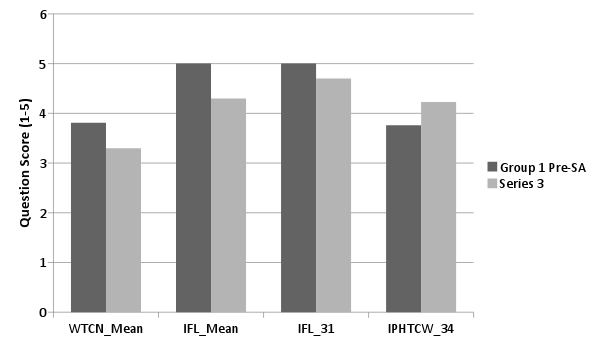
\includegraphics[width=6in,height=3.5in,width=\textwidth]{geoghegan-img1.png}
 \textit{Graph 2: Results of RQ1}
\end{styleNormali}


\begin{styleStandard}
In addition to comparing them to the Group 1 pre-SA students, the Group 2 end of SA students were also assessed using the comparison pairs ‘In General’ (IG) and ‘While Abroad’ (WA),wherein students reflected on how they felt about issues in general and specifically while abroad, as outlined in the methodology section. Results of Wilcoxon signed-rank tests showed that, of the 14 comparison pairs divided between ‘IG’ and ‘WA’, 4 pairs were statistically different (Table 4). 
\end{styleStandard}

\begin{flushleft}
\tablehead{}
\begin{supertabular}{m{0.38795984in}|m{1.4733598in}|m{1.5608599in}|m{0.63725984in}|m{0.46365985in}|m{0.37815985in}|m{0.5448598in}|}
\hline
\bfseries Pair &
\bfseries In General &
\bfseries While Abroad &
\bfseries \textit{T} &
\bfseries z &
\bfseries \textit{p} &
\bfseries \textit{n}\textit{\textsuperscript{2}}\\\hline
\mdseries 1 &
\mdseries 37. Using Eng/Fr/Ger in front of people in Spain makes me feel like I will be thought of as less Spanish. &
\mdseries 15. Using Eng/Fr/Ger in front of people on Erasmus makes me feel like I will be thought of as less Spanish. &
\mdseries 713.500 &
\mdseries 5.032 &
\mdseries .000 &
\mdseries 11.788\\\hline
\mdseries 2 &
\mdseries 53. If I could speak Eng/Fr/Ger well, I could get to know more people from other countries. &
\mdseries 26. If I could speak Eng/Fr/Ger well, I could get to know more people from other countries while on my Erasmus. &
\mdseries 41.000 &
\mdseries 3.624 &
\mdseries .000 &
\mdseries 11.596\\\hline
\mdseries 3 &
\mdseries 21. In the future, I would rather have a job in my home country than abroad. &
\mdseries 9. I would rather stay in my home country than live abroad. &
\mdseries 352.500 &
\mdseries 4.041 &
\mdseries .000 &
\mdseries 8.036\\\hline
\mdseries 4 &
\mdseries 16. I think I often feel anxious and ill at ease when I have to speak to someone in Eng/Fr/Ger. &
\mdseries 25. I think I often feel anxious and ill at ease when I have to speak Eng/Fr/Ger with a native speaker. &
\mdseries 313.000 &
{\mdseries 3.044}

 &
\mdseries .002 &
\mdseries 8.297\\\hline
\end{supertabular}
\end{flushleft}
\begin{styleStandard}
\textit{Table 4: Comparison Pairs}
\end{styleStandard}

\begin{styleStandard}
Pair 1 indicated that students felt they would be thought of as less Spanish when using their L2 in Spain as compared with on Erasmus. This suggests that students may perceive themselves to be more self-conscious about speaking their TL in their home country, given that they will not be presenting themselves as having a uniquely Spanish identity. On the other hand, in an international setting, students may perceive themselves as being free to exhibit their multilingual identity without threat. Pair 2 suggested that, while reflecting on being abroad, students were less inclined to think speaking their L2 well was needed to communicate with people from other countries, which seems counterintuitive. This could be explained by the fact that, while abroad, students may be exposed to more situations wherein they could use their TL, meaning that they did not need to seek out such situations to the extent they would at home. In other words, simply being abroad provided more opportunities to interact in the target language. This may have resulted in the students being less concerned with needing a high level in order to meet people from other countries: simply being abroad would lead to these opportunities. Pair 3 indicated that, in the future, students saw themselves working abroad more than simply living abroad. This suggests that students may have been more instrumentally motivated in this regard, thinking practically about their opportunities for economic advancement in the future. Pair 4 suggested that students were overall more anxious speaking to a native speaker while abroad, as opposed to any other speaker in the TL. This finding is consistent with what is suggested in the literature (e.g. Woodrow 2006).
\end{styleStandard}

\begin{listWWNumxxiileveli}
\item 
\setcounter{listWWNumxxiilevelii}{0}
\begin{listWWNumxxiilevelii}
\item 
\begin{stylelsSectionii}
RQ2: English vs. other languages
\end{stylelsSectionii}

\end{listWWNumxxiilevelii}
\end{listWWNumxxiileveli}
\begin{styleStandard}
The second research question in this study aimed to find whether there was an effect of a three-month study abroad on the motivation and identity of higher education students, sojourning in an English-speaking country as compared with a French or German speaking country\textit{.} In order to investigate this, Mann-Whitney U tests were also carried out in order to compare students who had sojourned, or planned to sojourn, in an English-speaking country with those in a German or French speaking country. Only 1 of the 14 categories, namely the Ideal L2 Self, and 4 individual questions, were found to be significantly different when comparing the two factors, which once again suggests caution in interpreting the results. Table 5 below shows the descriptive statistics with the means, the standard deviation and the test statistics for the category and questions which yielded significant results. 2 categories were relevant, namely the Ideal L2 Self (IL2S) and Intended Leaning Effort (ILE). Again, it should be borne in mind that higher values correspond to ‘strongly agree’ and ‘agree’ while lower values imply less agreement.
\end{styleStandard}

\begin{flushleft}
\tablehead{}
\begin{supertabular}{m{1.4872599in}|m{0.31705984in}|m{0.49835983in}|m{0.38935986in}|m{0.49835983in}|m{0.5344598in}|m{0.38935986in}|m{0.5441598in}|m{0.16435984in}|m{0.38795984in}|}
\hline
\bfseries Question &
\multicolumn{2}{m{0.8941598in}|}{\bfseries M} &
\multicolumn{2}{m{0.9664598in}|}{\bfseries SD} &
\bfseries \textit{U} &
\bfseries \textit{z} &
\bfseries \textit{p} &
\bfseries \textit{n}\textit{\textsuperscript{2}} &
\bfseries \textit{d}\\\hline
 &
\bfseries Eng &
\bfseries Fr/Ger &
\bfseries Eng &
\bfseries Fr/Ger &
 &
 &
 &
 &
\\\hline
\mdseries IL2S\_Mean &
\mdseries 4.57 &
\mdseries 3.58 &
\mdseries 1.05 &
\mdseries 1.60 &
\mdseries 216.000 &
\mdseries 2.597 &
\mdseries .009 &
\mdseries 0.057 &
\mdseries 0.49\\\hline
\mdseries IL2S\_42: In my future career, I imagine myself being able to use English/French/German. &
\mdseries 4.92 &
\mdseries 4.69 &
\mdseries .269 &
\mdseries .480 &
\mdseries 260.000 &
\mdseries 2.248 &
\mdseries .025 &
\mdseries 0.025 &
\mdseries 0.321\\\hline
\mdseries ILE\_24:It is extremely important for me to learn English/French/German. &
\mdseries 4.69 &
\mdseries 4.38 &
\mdseries .643 &
\mdseries .650 &
\mdseries 239.000 &
\mdseries 2.040 &
\mdseries .041 &
\mdseries 0.041 &
\mdseries 0.411\\\hline
\mdseries ILE\_4: If English/French/German were not taught in my home university, I would try to go to classes somewhere else. &
\mdseries 4.71 &
\mdseries 4.23 &
\mdseries .457 &
\mdseries .927 &
\mdseries 238.500 &
\mdseries 1.977 &
\mdseries .048 &
\mdseries 0.041 &
\mdseries 0.413\\\hline
\mdseries ILE\_54: If an English/French/German course was offered in the future, I would like to take it. &
\mdseries 4.04 &
\mdseries 4.69 &
\mdseries 1.120 &
\mdseries .480 &
\mdseries 453.000 &
\mdseries 2.044 &
\mdseries .041 &
\mdseries 0.055 &
\mdseries 0.481\\\hline
\end{supertabular}
\end{flushleft}
\begin{styleStandard}
[Warning: Draw object ignored][Warning: Draw object ignored]\textit{Table 5: Results of RQ2}
\end{styleStandard}

\begin{styleStandard}
Most importantly, the results show that the English group scored higher overall with regards to Ideal L2 Self (IL2S\_Mean), suggesting that those students focusing on learning English could better visualize themselves as the L2 user they wished to be than those in the Fr/Ger group. One reason for this could be the fact that the English group may simply see English having a greater part in their future, given its role as an international language. Within this category, it was found that those in the English group could imagine themselves using English in their future career (IL2S\_42) to a greater extent than the French /German group. This element of instrumental motivation is not surprising given the importance that is placed on speaking English for economic advancement, as mentioned above, and discussed by Block and Cameron (2002). Results also showed that while the English group were more likely to take classes elsewhere if it was not possible to learn their TL in their home university (ILE\_4), the French/German group were more likely to take a language course if it was offered in the future (ILE\_54). Finally, it was found that the English group were significantly more likely to think that it was extremely important for them to learn their target language (ILE\_24), again highlighting the importance placed on learning English. Graph 3 below displays the values above in order to offer a visual presentation of the results, where higher values correspond to more agreement with the proposed statements.
\end{styleStandard}

\begin{styleStandard}
  [Warning: Image ignored] % Unhandled or unsupported graphics:
%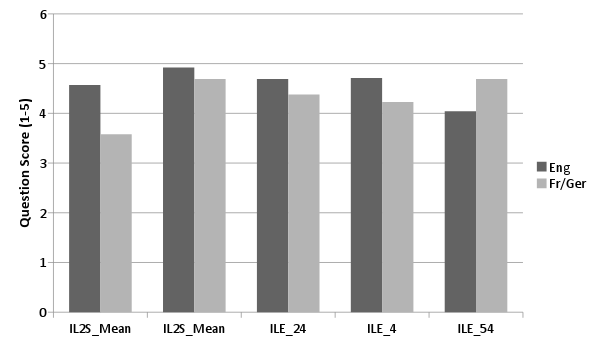
\includegraphics[width=6in,height=3.5in,width=\textwidth]{geoghegan-img2.png}
 
\end{styleStandard}

\begin{styleStandard}
\textit{Graph 3: Results of RQ2}
\end{styleStandard}

\begin{listWWNumxxiileveli}
\item 
\begin{stylelsSectioni}
Discussion
\end{stylelsSectioni}

\end{listWWNumxxiileveli}
\begin{styleStandard}
Regarding RQ1, the results of the questionnaire suggested a difference between Group 1 and 2 in 2 of the 14 categories, and a difference between the English and French/German subgroups of Group 2 in just 1 of the 14 categories. Results showed that the pre-SA Group 1 was significantly more likely to want to learn the foreign language of the country they will be visiting and that their overall mean for interest in foreign languages was greater than that of end of SA Group 2. Group 2, however, were significantly more likely to have thoughts they wish to share with others of different nationalities, suggesting a higher level of international posture in this regard. Finally, it was found that the pre-SA students were significantly more willing to communicate in their native language than in their target language, whereas the end of SA group were equally as likely to communicate in both languages. These findings are in keeping with the idea that SA offers a potential boost to the learner’s willingness to communicate, as well as a consequential development of a sense of belonging within an international community (Juan-Garau, Salazar-Noguera \& Prieto-Arranz 2014). Notably, regarding the remaining categories, no statistical difference was found, which suggests that a period of Study Abroad may have little or no effect on dimensions such as Fear of Assimilation, Instrumentality, Language Anxiety, L2 Self Confidence, International Vocation or Activities, Interest in International News and WTC in the TL. At this point, it should again be noted that in order to address this research question, a cross-sectional approach was taken. It is important to take this into consideration when discussing the results, and highlight the benefit of carrying out a similar study with a longitudinal approach in order to determine whether similar findings would arise. As for RQ2, comparing Group 2 students sojourning in an English-speaking country with those in a German- or French-speaking country, it was found that the English group considered learning their TL to be extremely important, and that students could imagine themselves using this language in their future careers a significantly greater amount than the other groups. In other words, as suggested in the literature, there is a tendency for those learning a lingua franca such as English to be increasingly instrumentally motivated (Block \& Cameron 2002). In addition, this group appeared to be better able to visualise themselves as the L2 users they wished to be than the French/German group, having a statistically higher score in the Ideal L2 Self mean. Finally, while the French/German group were more likely to take a language course if it was offered in the future, the English group were found to be more likely to take classes elsewhere (e.g. in a private language academy) if it was not possible to learn their TL in their home university. In these different ways, both groups appeared to show an interest in improving their formal language learning outside of the university setting. Again, despite these differences, a far greater number of categories showed no significant difference. This suggests that, while students who study in an English compared with a non-English speaking country may differ in particular with regards to the Ideal L2 Self, this appears not to be the case for the remaining dimensions. 
\end{styleStandard}

\begin{styleStandard}
The results of the questionnaire thus allow us to partially confirm our hypothesis, as only some categories resulted in a significant effect of a three-month SA on the language learning motivation and identity of higher education students, in particular regarding categories such as Willingness to Communicate in the native language, Interest in Foreign languages (comparing Pre-SA and end of SA, Research Question 1), and the Ideal L2 Self (comparing the English group with the French/German group, Research Question 2). 
\end{styleStandard}

\begin{styleStandard}
It is suggested that those questions which did not reach a statistical difference may not have done so due to two main reasons (besides the obvious possibility that our sample was not large enough to achieve sufficient statistical power). Firstly, it is possible that the instrument itself was unable to capture the subtle changes in the individual’s motivation and identity during study abroad or across groups. As is suggested by De Keyser (2014: 318), “much more detailed documentation is needed of how individual students are motivated for acquiring advanced language proficiency” and “how this motivation increases or decreases during their stay abroad”. Secondly, it is possible that there simply was no difference between the two groups, given that students in each group generally achieved very high scores in each section. As the students were all enrolled in specialised language learning degrees, it may be that the majority were just very highly motivated language learners, with no noticeable differences among the groups. This issue is also addressed by De Keyser (2014: 314), who points out that these language students who go on SA “are also quite motivated because language learning is what they are all about as translators/interpreters”. That is to say, there is a certain ceiling effect at hand, typical of learners at a more advanced stage (Meara 1994). It should also be pointed out that participation was entirely voluntary, meaning that it is possible that only those students who were more motivated participated in the study. Thus, while the findings of the study reveal some interesting differences among the various groups, what is perhaps more noteworthy is this lack of differences found in the majority of the categories. Categories such as Fear of Assimilation, Instrumentality, Language Anxiety, L2 Self Confidence, International Vocation or Activities, Interest in International News and WTC in the TL showed no statistical difference both overall, and in the individual questions. This is to say that neither the period of Study Abroad, nor the country which they studied in, affected these issues. Future research would benefit from investigating whether similar results would be found in a longitudinal study, and exploring the specific factors that affect, or do not affect, the student regarding the categories addressed in this study. 
\end{styleStandard}

\begin{listWWNumxxiileveli}
\item 
\begin{stylelsSectioni}
Conclusions
\end{stylelsSectioni}

\end{listWWNumxxiileveli}
\begin{styleStandard}
This study aimed to investigate the effect of SA on the motivation and identity of higher education students. The results show only a partial difference between the two groups who took the questionnaire, perhaps, as suggested above, due to the overall high levels of motivation across the students, indicating that a more detailed investigation is required in order to discern significant differences between the groups, if they do exist.
\end{styleStandard}

\begin{styleStandard}
Concerning the limitations of the study, besides the sample type, as already mentioned, a further issue was the sample size of students focusing on learning French or German. It was hoped that the groups would contain an equal number of students studying in each country; however, given the demand by students, the majority of placements were in English speaking countries.
\end{styleStandard}

\begin{styleStandard}
While individually the fields of SA, Identity, Motivation and ELF, as well as the theory of the L2 Motivational Self System, have been studied extensively, relatively little has been done so far to investigate how these elements interact. This study has taken the initial steps towards understanding the effect of a SA, on an array of factors pertaining to motivation and identity, investigating in particular elements from the L2 Motivational Self System, while also aiming to gain a preliminary understanding of the effect of ELF on these issues. It has been suggested that while a period of SA may have a positive impact on learners´ Willingness to Communicate in the NL and Interested in Foreign Languages, it may have no effect on the other issues that were investigated, as outlined above. Furthermore, comparing those studying abroad in an English/non-English speaking country, differences were found in particular with regards to the category of the Ideal L2 Self, with participants showing similarities in the other categories.
\end{styleStandard}

\begin{styleStandard}
As highlighted above, more detailed investigation is needed alongside the quantitative analysis, in order to fully understand and discern the similarities and differences between the groups. With this in mind, in order to gain a more thorough understanding of the development and negotiation of the learner’s ongoing motivational process during SA (Kim 2009), in Geoghegan and Pérez-Vidal (forthcoming), a follow-up study is carried out, adopting quantitative tools in order to provide this more detailed investigation. 
\end{styleStandard}

\begin{stylelsSectioni}
References
\end{stylelsSectioni}


\begin{styleStandard}
Aiken, Lewis. 1997. Questionnaires and inventories: Surveying opinions and assessing personality. New York: John Wiley.
\end{styleStandard}


\begin{styleStandard}
Allen, Heather Willis. 2010. Language-learning motivation during short-term study abroad: An activity theory perspective.~Foreign Language Annals~43(1). 27–49.
\end{styleStandard}


\begin{styleStandard}
Block, David. 2003.~The social turn in second language acquisition. Washington, DC: Georgetown University Press
\end{styleStandard}


\begin{styleStandard}
Block, David. 2006. Multilingual identities in a global city: London stories. London: Palgrave.
\end{styleStandard}


\begin{styleStandard}
Block, David. 2007. Second Language Identities. London/New York: Continuum.
\end{styleStandard}


\begin{styleStandard}
Bloomer, Aileen. 2010. Designing a questionnaire. In Susan Hunston \& David Oakley (eds.), Introducing applied linguistics concepts and skills (Vol. 13), 145–150. London: Routledge.
\end{styleStandard}


\begin{styleStandard}
Breiteneder, Angelika. 2005. Exploiting redundancy in English as a European lingua franca: the case of the ‘third person -s’. Vienna: University of Vienna. (Master’s Thesis.)
\end{styleStandard}


\begin{styleStandard}
British Council.~2013.~The English effect: The impact of English, what it{\textquotesingle}s worth to the UK and why it matters to the world. London: British Council. Clevedon: Multilingual Matters.
\end{styleStandard}


\begin{styleStandard}
Brown, Lucien. 2013. Identity and honori[FB01?]cs use in Korean study abroad.~In Celeste Kinginger (ed.), Social and cultural aspects of language learning in study abroad. 269–298.
\end{styleStandard}


\begin{styleStandard}
Coleman, James A. 1998. Language learning and study abroad: The European perspective.~Frontiers: The interdisciplinary journal of study abroad~4(2). 167–203.
\end{styleStandard}


\begin{styleStandard}
Coleman, James A. 2015. Social circles during residence abroad: What students do, and who with. In Rosamond Mitchell \& Nicole Tracy-Ventura \& Kevin McManus (eds.), Social interaction, identity and language learning during residence abroad, 33-52. Amsterdam: European Second Language Association.
\end{styleStandard}


\begin{styleStandard}
Collentine, Joseph G. \& Freed, Barbara F. 2004. Learning context and its effects on second language acquisition: Introduction.~Studies in second language acquisition~26(02). 153–171.
\end{styleStandard}


\begin{styleStandard}
Dailey, Aja. 2009. Key Motivational Factors and How Teachers Can Encourage Motivation in their Students. Birmingham: University of Birmingham. (Master’s Thesis.) 
\end{styleStandard}


\begin{styleStandard}
DeKeyser, Robert. 2014. Research on language development during study abroad. In Carmen Pérez-Vidal (ed.), Language acquisition in study abroad and formal instruction contexts, 313–325. Amsterdam: Benjamins.
\end{styleStandard}


\begin{styleStandard}
Devlin, Anne Marie. 2014. The impact of study abroad on the acquisition of sociopragmatic variation patterns: The case of non-native speaker English teachers. Intercultural Studies and Foreign Language Learning 13. Oxford: Peter Lang.
\end{styleStandard}


\begin{styleStandard}
Dörnyei, Zoltán. 2007. Research methods in applied linguistics. Oxford: Oxford University Press.
\end{styleStandard}


\begin{styleStandard}
Dörnyei, Zoltán. 2009. The L2 motivational self system. In Zoltán Dörnyei \& Ema Ushioda (eds.), Motivation, language identity and the L2 Self, 9–42. Bristol: Multilingual Matters.
\end{styleStandard}


\begin{styleStandard}
Dörnyei, Zoltán \& Csizér, Kata. 2012. How to design and analyze surveys in second language acquisition. In Alison Mackey \& Susan M. Gass (eds.), Research methods in second language acquisition: A practical guide, 74–94. Oxford: Wiley-Blackwell.
\end{styleStandard}


\begin{styleStandard}
Dörnyei, Zoltán \& Ottó, Istvan. 1998. Motivation in action: A process model of L2 motivation. Working Papers in Applied Linguistics 4. 43-69.
\end{styleStandard}


\begin{styleStandard}
Dörnyei, Zoltán \& Taguchi, Tatsuya. 2009.~Questionnaires in second language research: Construction, administration, and processing. London: Routledge.
\end{styleStandard}


\begin{styleStandard}
Dörnyei, Zoltán \& Ushioda, Ema. 2009. Motivation, language identities and the L2 self: a theoretical overview. In Zoltán Dörnyei \& Ema Ushioda (eds.), Motivation, language identity and the L2 self, 1–8. Bristol: Multilingual Matters. 
\end{styleStandard}


\begin{styleStandard}
Dörnyei, Zoltán \& Ushioda, Ema. 2013.~Teaching and researching: Motivation. London: Routledge.
\end{styleStandard}


\begin{styleStandard}
Gardner, Robert C. \& Lambert, Wallace E. 1972. Attitudes and motivation in second-language learning. Rowley: Newbury House Publishers
\end{styleStandard}


\begin{styleStandard}
Geoghegan, Leah. \& Pérez-Vidal, Carmen. Forthcoming. ELF, motivation and identity in SA. In %
%I cannot find this first name. There is nothing about this “forthcoming” book yet.
M. Howard (ed.), Study abroad, second language acquisition and interculturality: Contemporary perspectives. Bristol: Multilingual Matters.
\end{styleStandard}


\begin{styleStandard}
Guerrero, Mario. 2015. Motivation in second language learning: A historical overview and its relevance in a public high school in Pasto, Colombia.~HOW 22(1). 95–106.
\end{styleStandard}


\begin{styleStandard}
Hernández, Todd A. 2010. Promoting speaking proficiency through motivation and interaction: The study abroad and classroom learning contexts. Foreign Language Annals 43(4). 650–670.
\end{styleStandard}


\begin{styleStandard}
Higgins, E. Tory. 1987. Self-discrepancy: a theory relating self and affect. Psychological review~94(3). 319.
\end{styleStandard}


\begin{styleStandard}
%
%Not sure how LangSci wants websites to be done.
Identity [Def. 1]. 2016. In Oxford Dictionaries Online. Retrieved March 21, 2016, from \url{http://www.oxforddictionaries.com/definition/english/identity}
\end{styleStandard}


\begin{styleStandard}
Identity [Def. 2]. 2016. In Oxford Dictionaries Online. Retrieved March 21, 2016, from \url{http://www.oxforddictionaries.com/definition/english/identity}
\end{styleStandard}


\begin{styleStandard}
Irie, Kay \& Ryan, Stephen. 201. Study abroad and the dynamics of change in learner L2 self-concept. In Zoltán Dörnyei \& Peter D. MacIntyre \& Alastair Henry (eds.), Motivational dynamics in language learning, 343–366. Bristol: Multilingual Matters.
\end{styleStandard}


\begin{styleStandard}
Isabelli-García, Christina. 2006. Study abroad social networks, motivation and attitudes: Implications for second language acquisition. In Margaret A. DuFon \& Eton Churchill (eds.), Language learners in study abroad contexts, 231–258. Clevedon Multilingual Matters.
\end{styleStandard}


\begin{styleStandard}
Islam, Muhammad \& Lamb, Martin \& Chambers, Gary. 2013. The L2 motivational self-system and national interest: A Pakistani perspective.~System~41(2). 231–244.
\end{styleStandard}


\begin{styleStandard}
Jackson, Jane. 2008a. Globalization, internationalization, and short-term stays abroad.~International Journal of Intercultural Relations~32(4). 349–358.
\end{styleStandard}


\begin{styleStandard}
Jackson, Jane. 2008b.~Language, identity, and study abroad: Sociocultural perspectives. London: Equinox. 
\end{styleStandard}


\begin{styleStandard}
Jenkins, Jennifer. 2011. Accommodating (to) ELF in the international university. Journal of Pragmatics~43(4). 926–936.
\end{styleStandard}


\begin{styleStandard}
Jenkins, Jennifer \& Cogo, Alessia \& Dewey, Martin. 2011. Review of developments in research into English as a lingua franca. Language Teaching 44(3). 281–315. 
\end{styleStandard}


\begin{styleStandard}
Juan-Garau, Maria \& Salazar-Noguera, Juana \& Prieto-Arranz, José Igor. 2014. English L2 learners’ lexico-grammatical and motivational development at home and abroad. In Carmen Pérez-Vidal (ed.),~Language acquisition in study abroad and formal instruction contexts, 235–258. Amsterdam: John Benjamins Publishing Company.
\end{styleStandard}


\begin{styleStandard}
Kalocsai, Karolina. 2011. The show of interpersonal involvement and the building of rapport in an ELF community of practice. In Alasdair Archibald \& Alesia Cogo \& Jennifer Jenkins (eds.),~Latest trends in English as a lingua franca research, 113-138. Newcastle upon Tyne: Cambridge Scholars Publishing.
\end{styleStandard}


\begin{styleStandard}
Kaypak, Eda \& Ortaçtepe, Deniz. 2014. Language learner beliefs and study abroad: A study on English as a lingua franca (ELF).~System~42. 355–367
\end{styleStandard}


\begin{styleStandard}
Ke, I-Chung \& Cahyani, Hilda. 2014. Learning to become users of English as a Lingua Franca (ELF): How ELF online communication affects Taiwanese learners{\textquotesingle} beliefs of English.~System~46. 28–38.
\end{styleStandard}


\begin{styleStandard}
Kim, Tae-Young. 2009. The dynamics of L2 self and L2 learning motivation[202F?]: A qualitative case study of Korean ESL students. English Teaching 64(3). 49–70.
\end{styleStandard}


\begin{styleStandard}
Kim, Tae-Young \& Kim, Yoon-Kyoung. 2014. A structural model for perceptual learning styles, the ideal l2 self, motivated behavior, and English proficiency. System 46. 14–27.
\end{styleStandard}


\begin{styleStandard}
Kinginger, Celeste. 2004. Alice doesn’t live here anymore: foreign language learning and identity construction. In A. Pavlenko \& A. Blackledge (eds.), Negotiation of Identities in Multilingual Contexts. Cleveden, 219–242. Bristol: Multilingual Matters.
\end{styleStandard}


\begin{styleStandard}
Kinginger, Celeste. 2013. Identity and language learning in study abroad.~Foreign Language Annals 46(3). 339–358.
\end{styleStandard}


\begin{styleStandard}
Larson-Hall, Jenifer. 2012. How to run statistical analyses. In Alison Mackey \& Susan M. Gass (eds.), Research methods in second language acquisition: A practical guide, 245–274. Oxford: Wiley-Blackwell.
\end{styleStandard}


\begin{styleStandard}
Macksoud, Ruby. 2010. Using interview data in case studies. In Susan Hunston \& David Oakley (eds.), Introducing applied linguistics: Concepts and skills, 153–159. London: Routledge.
\end{styleStandard}


\begin{styleStandard}
Majanen, Silke. 2008. English as a lingua franca[202F?]: Teachers’ discourses on accent and identity. Helsinki: University of Helsinki. (Master’s Thesis.) 
\end{styleStandard}


\begin{styleStandard}
Markus, Hazel \& Nurius, Paula Goodstein. 1986. Possible selves.~American psychologist 41(9). 954–969.
\end{styleStandard}


\begin{styleStandard}
Mazzarol, Tim \& Norman Soutar, Geoffrey \& Sim Yaw Seng, Michael. 2003. The third wave: Future trends in international education.~International Journal of Educational Management~17(3). 90–99.
\end{styleStandard}


\begin{styleStandard}
Melitz, Jacques. 2016. English as a global language. In~Victor Ginsburgh \& Shlomo Weber (eds.) The Palgrave handbook of economics and language, pp. 583–615. Houndmill: Palgrave Macmillan UK.
\end{styleStandard}


\begin{styleStandard}
Mitchell, Rosamond \& Tracy-Ventura, Nicole \& McManus, Kevin. 2015. Introduction. In Rosamond Mitchell \& Nicole Tracy-Ventura \& Kevin McManus (eds.), Social interaction, identity and language learning during residence abroad, 7–13. Amsterdam: European Second Language Association..
\end{styleStandard}


\begin{styleStandard}
Mitchell, R. \& McManus, K. \& Tracy-Ventura, N. 2015. Placement type and language learning during residence abroad. In Rosamond Mitchell \& Nicole Tracy-Ventura \& Kevin McManus (eds.), Social interaction, identity and language learning during residence abroad, 115–138. Amsterdam: European Second Language Association.
\end{styleStandard}


\begin{styleStandard}
Nestor, Niamh\& Regan, Vera. 2011. The new kid on the block. A case study of young Poles, language and identity. In Merike Darmody \& Naomi Tyrrell \& S. Song (eds.), The changing faces of Ireland: Exploring the live of immigrant and ethnic minority children, 35–52. Rotterdam: Sense Publishers.
\end{styleStandard}


\begin{styleStandard}
Nestor, Niamh \& Ní Chasaide, Caitríona \& Regan, Vera. 2012. Discourse ‘like’ and social identity – a case study of Poles in Ireland. In Bettina Migge \& Máire Ní Chiosáin (eds.), New perspectives on Irish English, 327–354. Amsterdam: John Benjamins.
\end{styleStandard}


\begin{styleStandard}
Norton, Bonny. 2000. Identity and Language Learning. London: Longman.
\end{styleStandard}


\begin{styleStandard}
Pakir, Anne. 2009. English as a lingua franca: Analyzing research frameworks in international English, world Englishes, and ELF.~World Englishes 28(2). 224–235.
\end{styleStandard}


\begin{styleStandard}
Papi, Mostafa. 2010. The L2 motivational self system, L2 anxiety, and motivated behavior: A structural equation modeling approach. System 38(3). 467–479.
\end{styleStandard}


\begin{styleStandard}
Pérez-Vidal, Carmen. 2011. Language acquisition in three different contexts of learning: Formal instruction, study abroad and semi-immersion (CLIL). In Yolanda Ruiz de Zarobe \& Juan Manuel Sierra \& Francisco Gallardo del Puerto (eds.),\textbf{~}Content and foreign language integrated learning: Contributions to multilingualism in European contexts, 25–35. Bern/Berlin: Peter Lang.
\end{styleStandard}


\begin{styleStandard}
Regan, Vera. 2013. The bookseller and the basketball player: tales from the French Polonia. In David Singleton \& Vera Regan \& Ewelina Debaene (eds.), Linguistic and cultural acquisition in a migrant community, 28–48. Bristol: Multilingual Matters. 
\end{styleStandard}


\begin{styleStandard}
Ryan, Stephen. 2009. Self and identity in L2 motivation in Japan: The ideal L2 self and Japanese learners of English. In Zoltán Dörnyei \& Ema Ushioda (eds.), Motivation, language identity and the L2 self, 120–143. Bristol: Multilingual Matters.
\end{styleStandard}


\begin{styleStandard}
Sasaki, Miyuki. 2011. Effects of varying lengths of study-abroad experiences on Japanese EFL students’ L2 writing ability and motivation: A longitudinal study. TESOL Quarterly 45(1). 81–105.
\end{styleStandard}


\begin{styleStandard}
Seidlhofer, Barbara. 2001. Closing a conceptual gap: The case for a description of English as a lingua franca.~International Journal of Applied Linguistics~11(2). 133–158.
\end{styleStandard}


\begin{styleStandard}
Smit, Ute. 2010.~English as a lingua franca in higher education: A longitudinal study of classroom discourse~(Vol. 2). Berlin: Mouton de Gruyter.
\end{styleStandard}


\begin{styleStandard}
Stockton, Heather Lynn (2015). Identity-focused second language acquisition[202F?]: a systematic review of classroom applications. St. Paul: Hamline University. (Master’s Thesis.) 
\end{styleStandard}


\begin{styleStandard}
Taguchi, Tatsuya \& Magid, Michael \& Papi, Mostafa. 2009. The L2 motivational self system among Japanese, Chinese and Iranian learners of English: A comparative study. In Zoltán Dörnyei \& Ema Ushioda (eds.), Motivation, language identity and the L2 self, 66–97. Bristol: Multilingual Matters.
\end{styleStandard}


\begin{styleStandard}
Ushioda, Ema 2009. A person-in-context relational view of emergent motivation, self and identity. In Zoltán Dörnyei \& Ema Ushioda (eds.), Motivation, language identity and the L2 self, 215–228. Bristol: Multilingual Matters.
\end{styleStandard}


\begin{styleStandard}
Ushioda, Ema \& Dörnyei, Zoltán. 2012. Motivation. In Susan Gass \& Alison Mackey (eds.),~The Routledge handbook of second language acquisition, 396–409. New York: Routledge
\end{styleStandard}


\begin{styleStandard}
Waninge, Freekien \& Dörnyei, Zoltán \& De Bot, Kees 2014. Motivational dynamics in language learning: Change, stability, and context. Modern Language Journal 98(3). 704–723. 
\end{styleStandard}


\begin{styleStandard}
Wenger, Etienne. 1998.~Communities of practice: Learning, meaning, and identity. Cambridge: Cambridge University Press.
\end{styleStandard}


\begin{styleStandard}
Woodrow, Lindy. 2006. Anxiety and speaking English as a second language.~RELC Journal: A Journal of Language Teaching and Research~37(3). 308–328.
\end{styleStandard}


\begin{styleStandard}
Yashima, Tomoko. 2009. International posture and the ideal L2 self in the Japanese EFL context. In~Zoltán Dörnyei \& Ema Ushioda (eds.), Motivation, language identity and the L2 self, 144–163. Bristol: Multilingual Matters.
\end{styleStandard}


\begin{stylelsSectioni}
Appendix 1: Questionnaire Content
\end{stylelsSectioni}


\begin{styleStandard}
We would like to ask you to help us by answering the following questions~concerning language learning in Study Abroad, and people{\textquotesingle}s feelings about languages and communication in general. This is not a test so there are no “right” or “wrong” answers. We are interested in your personal opinion. Please give your answers sincerely as only this will guarantee the success of the investigation. Thank you very much for your help!~
\end{styleStandard}

\begin{stylelsSectionii}
Section 1. 
\end{stylelsSectionii}


\begin{styleStandard}
\textbf{First, would you please answer a few personal details and general information – we need this information to be able to interpret your answers properly. }
\end{styleStandard}

\setcounter{listWWNumxxxleveli}{0}
\begin{listWWNumxxxleveli}
\item 
\begin{stylelsEnumerated}
What is your name?
\end{stylelsEnumerated}

\end{listWWNumxxxleveli}
\setcounter{listWWNumxleveli}{0}
\begin{listWWNumxleveli}
\item 
\begin{stylelsEnumerated}
What is your age (in years)?
\end{stylelsEnumerated}

\item 
\begin{stylelsEnumerated}
What degree are you studying?
\end{stylelsEnumerated}

\item 
\begin{stylelsEnumerated}
What foreign languages are you studying as part of your degree? Please write the language, how old you were when you started learning, and your level. e.g. English (6, B2.2) = (I am learning English. I started learning English when I was 6 years old. My level is B2.2) French (11, B1.1) = (I am learning French. I started learning French when I was 11 years old. My level is B1.1)
\end{stylelsEnumerated}

\item 
\begin{stylelsEnumerated}
In what country are you doing your Erasmus?
\end{stylelsEnumerated}

\item 
\begin{stylelsEnumerated}
Why did you choose this country/language to do your Erasmus?
\end{stylelsEnumerated}

\item 
\begin{stylelsEnumerated}
Before this Erasmus, had you ever spent a period of time in a foreign country? If yes, where and for how long (in weeks)? Please include all trips .e.g. 1. England (2 weeks) summer 2010,~2. England (4 weeks) summer 2011, 3. Germany (1 week) summer family trip 2011, etc.
\end{stylelsEnumerated}

\end{listWWNumxleveli}
\begin{stylelsSectionii}
Section 2
\end{stylelsSectionii}


\begin{styleStandard}
\textbf{In this section, there are going to be questions concerning interpersonal communication in everyday and classroom situations, using your native language, or the language you are learning. In some questions, you will be given the option English/French/German.~Please answer ONLY with regards to the language of the country where you are abroad (i.e. French if you are in France, German if you are in Germany or English if you are in an English-speaking country).}
\end{styleStandard}

\begin{styleStandard}
Q1. How likely would you be to initiate communication in your native language in the following situations?
\end{styleStandard}

\setcounter{listWWNumxxxileveli}{0}
\begin{listWWNumxxxileveli}
\item 
\begin{stylelsEnumerated}
1.Talking with an acquaintance while waiting for the bus (2)
\end{stylelsEnumerated}

\end{listWWNumxxxileveli}
\setcounter{listWWNumxleveli}{0}
\begin{listWWNumxleveli}
\item 
\begin{stylelsEnumerated}
2.Talking with a salesperson in a store. (3)
\end{stylelsEnumerated}

\item 
\begin{stylelsEnumerated}
3.Talking in a small group of strangers. (4)
\end{stylelsEnumerated}

\item 
\begin{stylelsEnumerated}
4.Talking with a friend while waiting for the bus (5)
\end{stylelsEnumerated}

\item 
\begin{stylelsEnumerated}
5.Talking with a stranger while waiting for the bus (6)
\end{stylelsEnumerated}

\item 
\begin{stylelsEnumerated}
6.Talking in a small group of acquaintances. (7)
\end{stylelsEnumerated}

\item 
\begin{stylelsEnumerated}
7.Volunteering to make a presentation in front of a large group (8)
\end{stylelsEnumerated}

\item 
\begin{stylelsEnumerated}
8.Being the first one to speak while doing group work (9)
\end{stylelsEnumerated}

\item 
\begin{stylelsEnumerated}
9.Asking the teacher a question in front of the class (10)
\end{stylelsEnumerated}

\end{listWWNumxleveli}
\begin{styleStandard}
Q2. How likely would you be to initiate communication in English/French/German in the following situations?
\end{styleStandard}

\setcounter{listWWNumxxxiileveli}{0}
\begin{listWWNumxxxiileveli}
\item 
\begin{stylelsEnumerated}
1.Talking with an acquaintance while waiting for the bus (2)
\end{stylelsEnumerated}

\end{listWWNumxxxiileveli}
\setcounter{listWWNumxleveli}{0}
\begin{listWWNumxleveli}
\item 
\begin{stylelsEnumerated}
2.Talking with a salesperson in a store. (3)
\end{stylelsEnumerated}

\item 
\begin{stylelsEnumerated}
3.Talking in a small group of strangers. (4)
\end{stylelsEnumerated}

\item 
\begin{stylelsEnumerated}
4.Talking with a friend while waiting for the bus (5)
\end{stylelsEnumerated}

\item 
\begin{stylelsEnumerated}
5.Talking with a stranger while waiting for the bus (6)
\end{stylelsEnumerated}

\item 
\begin{stylelsEnumerated}
6.Talking in a small group of acquaintances. (7)
\end{stylelsEnumerated}

\item 
\begin{stylelsEnumerated}
7.Volunteering to make a presentation in front of a large group (1)
\end{stylelsEnumerated}

\item 
\begin{stylelsEnumerated}
8.Being the first one to speak while doing group work (8)
\end{stylelsEnumerated}

\item 
\begin{stylelsEnumerated}
9.Asking the teacher a question in front of the class (9)
\end{stylelsEnumerated}

\end{listWWNumxleveli}
\begin{styleStandard}
Q3. This section is about the importance and usefulness of languages in the world.
\end{styleStandard}

\setcounter{listWWNumxxxiiileveli}{0}
\begin{listWWNumxxxiiileveli}
\item 
\begin{stylelsEnumerated}
1.How much do you think knowing English/French/German would help you to become a more knowledgeable person? (1)
\end{stylelsEnumerated}

\end{listWWNumxxxiiileveli}
\setcounter{listWWNumxleveli}{0}
\begin{listWWNumxleveli}
\item 
\begin{stylelsEnumerated}
2.How much do you think English/French/German would help you if you travelled abroad in the future? (2)
\end{stylelsEnumerated}

\item 
\begin{stylelsEnumerated}
3.How much do you think English/French/German would help your future career? (3)
\end{stylelsEnumerated}

\item 
\begin{stylelsEnumerated}
4.To what extent do you think English/French/German is important in the world these days? (4)
\end{stylelsEnumerated}

\end{listWWNumxleveli}
\begin{stylelsSectionii}
Section 3.1. 
\end{stylelsSectionii}


\begin{styleStandard}
\textbf{Finally, in this last section, we would like to know to what extent the statements included describe your own feelings or~situation. After each statement you’ll find five options. Please select the option~which best expresses how true the statement is about your feelings or situation.~For example, if the first~statement~was {\textquotedbl}I like skiing{\textquotedbl} and you like skiing very much, select the first~option. Remember: In some questions, you will be given the option English/French/German.~Please answer ONLY with regards to the language of the country where you are abroad (i.e. French if you are in France, German if you are in Germany or English if you are in an English-speaking country). First, think about how you feel while you are studying abroad and answering this questionnaire.}
\end{styleStandard}

\setcounter{listWWNumxxixleveli}{0}
\begin{listWWNumxxixleveli}
\item 
\begin{stylelsEnumerated}
1. While abroad, I take every opportunity I can to speak English/French/German with international friends. (66)
\end{stylelsEnumerated}

\end{listWWNumxxixleveli}
\setcounter{listWWNumxleveli}{0}
\begin{listWWNumxleveli}
\item 
\begin{stylelsEnumerated}
2. I’m not very good at volunteering answers in my classes in English/French/German. (67)
\end{stylelsEnumerated}

\item 
\begin{stylelsEnumerated}
3. I often read newspapers and watch tv news in the language of the country I am staying (68)
\end{stylelsEnumerated}

\item 
\begin{stylelsEnumerated}
4. I think that my writing ability has improved the most during this Erasmus (88)
\end{stylelsEnumerated}

\item 
\begin{stylelsEnumerated}
5. When I first arrived, I found it more difficult to learn English/French/German while on Erasmus than while at home. (69)
\end{stylelsEnumerated}

\item 
\begin{stylelsEnumerated}
6. When I first arrived, I found it more difficult to learn English/French/German than halfway through my Erasmus (93)
\end{stylelsEnumerated}

\item 
\begin{stylelsEnumerated}
7. I am worried that other speakers of English/French/German would find my English/French/German strange. (70)
\end{stylelsEnumerated}

\item 
\begin{stylelsEnumerated}
8. I try to avoid talking with native English/French/German speakers if I can (71)
\end{stylelsEnumerated}

\item 
\begin{stylelsEnumerated}
9. I would rather stay in my home country than live abroad. (72)
\end{stylelsEnumerated}

\item 
\begin{stylelsEnumerated}
10. I would not like to live with someone of a different nationality than me. (73)
\end{stylelsEnumerated}

\item 
\begin{stylelsEnumerated}
11. Halfway through my Erasmus, I thought it was easier to learn English/French/German abroad than at home (74)
\end{stylelsEnumerated}

\item 
\begin{stylelsEnumerated}
12. I think I would be studying English/French/German even if it weren’t compulsory. (75)
\end{stylelsEnumerated}

\item 
\begin{stylelsEnumerated}
13. I worry that native speakers will laugh at me when I speak English/French/German. (76)
\end{stylelsEnumerated}

\item 
\begin{stylelsEnumerated}
14.I think that my reading ability has improved the most during this Erasmus (92)
\end{stylelsEnumerated}

\item 
\begin{stylelsEnumerated}
15. Using English/French/German in front of people on Erasmus makes me feel like I will be thought of as less Spanish. (77)
\end{stylelsEnumerated}

\item 
\begin{stylelsEnumerated}
16. I think I often feel anxious and ill at ease when I have to speak to someone in English/French/German (78)
\end{stylelsEnumerated}

\item 
\begin{stylelsEnumerated}
17. I would get tense if someone asked me for directions in English/French/German. (79)
\end{stylelsEnumerated}

\item 
\begin{stylelsEnumerated}
18. I think that my speaking ability has improved the most during this Erasmus (89)
\end{stylelsEnumerated}

\item 
\begin{stylelsEnumerated}
19. Whenever I think of my future career, I imagine myself being able to use English/French/German. (80)
\end{stylelsEnumerated}

\item 
\begin{stylelsEnumerated}
20. I think that my listening ability has improved the most during this Erasmus (90)
\end{stylelsEnumerated}

\item 
\begin{stylelsEnumerated}
21. I’m interested in the news of the country where I’m staying. (81)
\end{stylelsEnumerated}

\item 
\begin{stylelsEnumerated}
22. In the future, I want to work in a foreign country. (82)
\end{stylelsEnumerated}

\item 
\begin{stylelsEnumerated}
23. I get nervous and confused when I am speaking in my English/French/German classes. (83)
\end{stylelsEnumerated}

\item 
\begin{stylelsEnumerated}
24. I think that my pronunciation has improved the most during this Erasmus (91)
\end{stylelsEnumerated}

\item 
\begin{stylelsEnumerated}
25. I can honestly say that I am really doing my best to learn English/French/German while on my Erasmus (84)
\end{stylelsEnumerated}

\item 
\begin{stylelsEnumerated}
26. If I could speak English/French/German well, I could get to know more people from other countries while on my Erasmus (85)
\end{stylelsEnumerated}

\item 
\begin{stylelsEnumerated}
27. English/French/German ability would help me get a better paying job. (86)
\end{stylelsEnumerated}

\item 
\begin{stylelsEnumerated}
28. Now that I{\textquotesingle}m at the end of my Erasmus, I think it is easier to learn English/French/German at home than abroad. (87)
\end{stylelsEnumerated}

\item 
\begin{stylelsEnumerated}
29. Now that I{\textquotesingle}m at the end of my Erasmus, I think that it is more difficult to learn English/French German than I did halfway through. (94)
\end{stylelsEnumerated}

\item 
\begin{stylelsEnumerated}
30. I am more eager to return home now than I was halfway through my Erasmus. (95)
\end{stylelsEnumerated}

\end{listWWNumxleveli}
\begin{stylelsSectionii}
Section 3.2
\end{stylelsSectionii}


\begin{styleStandard}
\textbf{Now, think about how you feel IN GENERAL about each of these statements.}
\end{styleStandard}

\setcounter{listWWNumxxviiileveli}{0}
\begin{listWWNumxxviiileveli}
\item 
\begin{stylelsEnumerated}
1. I often read newspapers and watch TV news about foreign countries (123)
\end{stylelsEnumerated}

\end{listWWNumxxviiileveli}
\setcounter{listWWNumxleveli}{0}
\begin{listWWNumxleveli}
\item 
\begin{stylelsEnumerated}
54. If an English/French/German course was offered in the future, I would like to take it. (177)
\end{stylelsEnumerated}

\item 
\begin{stylelsEnumerated}
2. If I made the effort, I could learn a new foreign language. (124)
\end{stylelsEnumerated}

\item 
\begin{stylelsEnumerated}
3. I would feel somewhat uncomfortable if a foreigner moved in next door. (125)
\end{stylelsEnumerated}

\item 
\begin{stylelsEnumerated}
4. If English/French/German were not taught in my home university, I would try to go to classes somewhere else. (126)
\end{stylelsEnumerated}

\item 
\begin{stylelsEnumerated}
5. I can imagine speaking English/French/German with international friends in my home country. (127)
\end{stylelsEnumerated}

\item 
\begin{stylelsEnumerated}
6. I’m not very good at volunteering answers in our English/French/German language class in my home university. (128)
\end{stylelsEnumerated}

\item 
\begin{stylelsEnumerated}
7. When I hear a song in English/French/German, I listen carefully and try to understand all the words. (129)
\end{stylelsEnumerated}

\item 
\begin{stylelsEnumerated}
8. Learning a foreign language is a difficult task for me. (130)
\end{stylelsEnumerated}

\item 
\begin{stylelsEnumerated}
9. I have ideas about international issues, such as environmental issues and north-south issues. (131)
\end{stylelsEnumerated}

\item 
\begin{stylelsEnumerated}
10. I would like to be able to use English/French/German to get involved with people from other countries. (132)
\end{stylelsEnumerated}

\item 
\begin{stylelsEnumerated}
11. In the future, I would like to make friends with international students studying in my home country. (133)
\end{stylelsEnumerated}

\item 
\begin{stylelsEnumerated}
12. As a part of international society Spanish people must preserve the Spanish language and culture. (134)
\end{stylelsEnumerated}

\item 
\begin{stylelsEnumerated}
13. I have issues to address with people from different parts of the world (135)
\end{stylelsEnumerated}

\item 
\begin{stylelsEnumerated}
14. I am sure I will be able to learn English/French/German to a high level. (136)
\end{stylelsEnumerated}

\item 
\begin{stylelsEnumerated}
15. Learning English/French/German is necessary because it is an international language (137)
\end{stylelsEnumerated}

\item 
\begin{stylelsEnumerated}
16. Studying English/French/German will help me get a good job (138)
\end{stylelsEnumerated}

\item 
\begin{stylelsEnumerated}
17. I always feel that my classmates speak English/French/German better than I do. (139)
\end{stylelsEnumerated}

\item 
\begin{stylelsEnumerated}
18. I don{\textquotesingle}t think what{\textquotesingle}s happening overseas has much to do with my daily life. (140)
\end{stylelsEnumerated}

\item 
\begin{stylelsEnumerated}
19. As internationalization advances there is a danger of losing the Spanish language and culture. (141)
\end{stylelsEnumerated}

\item 
\begin{stylelsEnumerated}
20. When I think about my future, it is important that I use English/French/German. (142)
\end{stylelsEnumerated}

\item 
\begin{stylelsEnumerated}
21. In the future, I would rather have a job in my home country than abroad. (143)
\end{stylelsEnumerated}

\item 
\begin{stylelsEnumerated}
22. I think that English/French/German will help me meet more people (144)
\end{stylelsEnumerated}

\item 
\begin{stylelsEnumerated}
23. I would like to be able to use English/French/German to communicate with people from other countries. (145)
\end{stylelsEnumerated}

\item 
\begin{stylelsEnumerated}
24. It is extremely important for me to learn English/French/German. (146)
\end{stylelsEnumerated}

\item 
\begin{stylelsEnumerated}
25. I feel uneasy speaking English/French/German with a native speaker. (147)
\end{stylelsEnumerated}

\item 
\begin{stylelsEnumerated}
26. I have a strong interest in international affairs. (148)
\end{stylelsEnumerated}

\item 
\begin{stylelsEnumerated}
27. The things I want to do in the future require me to speak English/French/German. (149)
\end{stylelsEnumerated}

\item 
\begin{stylelsEnumerated}
28. If my dreams come true, I will use English/French/German effectively in the future. (150)
\end{stylelsEnumerated}

\item 
\begin{stylelsEnumerated}
29. I wouldn{\textquotesingle}t mind sharing an apartment or room with an international student. (151)
\end{stylelsEnumerated}

\item 
\begin{stylelsEnumerated}
30. As a result of internationalization, there is a danger Spanish people may forget the importance of Spanish culture. (152)
\end{stylelsEnumerated}

\item 
\begin{stylelsEnumerated}
31. If I were visiting a foreign country I would like to be able to speak its language. (153)
\end{stylelsEnumerated}

\item 
\begin{stylelsEnumerated}
32. Studying English/French/German will give me more opportunities. (154)
\end{stylelsEnumerated}

\item 
\begin{stylelsEnumerated}
33. In the future, I would like to participate in a volunteer activity to help foreigners living in the surrounding community (155)
\end{stylelsEnumerated}

\item 
\begin{stylelsEnumerated}
34. I have thoughts that I want to share with people from other parts of the world. (156)
\end{stylelsEnumerated}

\item 
\begin{stylelsEnumerated}
35. I think I would study a foreign language even if it weren’t compulsory. (157)
\end{stylelsEnumerated}

\item 
\begin{stylelsEnumerated}
36. I worry that the other students will laugh at me when I speak English/French/German. (158)
\end{stylelsEnumerated}

\item 
\begin{stylelsEnumerated}
37. Using English/French/German in front of people in Spain makes me feel like I will be thought of as less Spanish. (159)
\end{stylelsEnumerated}

\item 
\begin{stylelsEnumerated}
38. A knowledge of English/French/German would make me a better educated person. (160)
\end{stylelsEnumerated}

\item 
\begin{stylelsEnumerated}
39. I would like to learn a lot of foreign languages. (161)
\end{stylelsEnumerated}

\item 
\begin{stylelsEnumerated}
40. I would talk to an international student if there was one in my class in my home university. (162)
\end{stylelsEnumerated}

\item 
\begin{stylelsEnumerated}
41. When I meet a speaker of English/French/German, I feel nervous. (163)
\end{stylelsEnumerated}

\item 
\begin{stylelsEnumerated}
42. In my future career, I imagine myself being able to use English/French/German. (164)
\end{stylelsEnumerated}

\item 
\item 
\begin{stylelsEnumerated}
43. I often imagine myself as someone who is able to speak English/French/German. (165)
\end{stylelsEnumerated}

\item 
\begin{stylelsEnumerated}
44. I{\textquotesingle}m not much interested in overseas news. (166)
\end{stylelsEnumerated}

\item 
\begin{stylelsEnumerated}
45. If I could have access to TV stations in English/French/German, I would try to watch them often. (167)
\end{stylelsEnumerated}

\item 
\begin{stylelsEnumerated}
46. I am the kind of person who makes great efforts to learn English/French/German. (168)
\end{stylelsEnumerated}

\item 
\begin{stylelsEnumerated}
47. I{\textquotesingle}m interested in an international career in the future (169)
\end{stylelsEnumerated}

\item 
\begin{stylelsEnumerated}
48. For me to become an educated person, I should learn English/French/German. (170)
\end{stylelsEnumerated}

\item 
\begin{stylelsEnumerated}
49. I have no clear opinions about international issues. (171)
\end{stylelsEnumerated}

\item 
\begin{stylelsEnumerated}
50. I want to work in an international organization such as the United Nations. (172)
\end{stylelsEnumerated}

\item 
\begin{stylelsEnumerated}
51. I often talk about situations and events in foreign countries with my family and/or friends. (173)
\end{stylelsEnumerated}

\item 
\begin{stylelsEnumerated}
52. I can honestly say that I am really doing my best to learn English/French/German. (174)
\end{stylelsEnumerated}

\item 
\begin{stylelsEnumerated}
53. If I could speak English/French/German well, I could get to know more people from other countries. (175)
\end{stylelsEnumerated}

\item 
\begin{stylelsEnumerated}
55. I am working hard at learning English/French/German. (178)
\end{stylelsEnumerated}

\item 
\begin{stylelsEnumerated}
6. In the future, English/French/German ability would help me get a better paying job. (179)
\end{stylelsEnumerated}

\end{listWWNumxleveli}
\begin{stylelsSectioni}
Appendix 2: Cronbach Alpha Values
\end{stylelsSectioni}


\begin{flushleft}
\tablehead{}
\begin{supertabular}{|m{1.1212599in}|m{1.1212599in}|m{1.1212599in}|m{1.1212599in}|m{1.1219599in}|}
\hline
\bfseries Category  &
\bfseries Number of Items &
\bfseries Cronbach Alpha (Original Study) &
\bfseries Number of Items &
{\bfseries Cronbach Alpha}

\bfseries (This Study)\\\hline
\mdseries Fear of Assimilation  &
\mdseries 4 &
\mdseries \textit{$\alpha $ =0.67 } &
\mdseries 4 &
\mdseries \textit{$\alpha $ =}0.651\\\hline
\mdseries Ideal L2 Self  &
\mdseries 6 &
\mdseries \textit{$\alpha $=0.85 } &
\mdseries 4 &
\mdseries \textit{$\alpha $ =}0.761\\\hline
\mdseries Instrumentality  &
\mdseries 6 &
\mdseries \textit{$\alpha $ =0.87 } &
\mdseries 6 &
\mdseries \textit{$\alpha $ =}0.759\\\hline
\mdseries Intended Learning Effort  &
\mdseries 8 &
\mdseries \textit{$\alpha $ =0.86 } &
\mdseries 8 &
\mdseries \textit{$\alpha $ =}0.760\\\hline
\mdseries Interest in Foreign Languages  &
\mdseries 4 &
\mdseries \textit{$\alpha $ =0.70 } &
\mdseries 3 &
\mdseries \textit{$\alpha $ =}0.629\\\hline
\mdseries International Contact  &
\mdseries 4 &
\mdseries \textit{$\alpha $ =0.87 } &
\mdseries 4 &
\mdseries \textit{$\alpha $ =}0.609\\\hline
\mdseries Language Anxiety  &
\mdseries 3 &
\mdseries \textit{$\alpha $ =0.81 } &
\mdseries 3 &
\mdseries \textit{$\alpha $ =} 0.670\\\hline
\mdseries L2 Self Confidence  &
\mdseries 4 &
\mdseries \textit{$\alpha $ =0.57 } &
\mdseries 3 &
\mdseries \textit{$\alpha $ =}0.625\\\hline
\mdseries Willingness to Communicate Native Language &
\mdseries 9 &
\mdseries \textit{$\alpha $ =0.87 } &
\mdseries 9 &
\mdseries \textit{$\alpha $ =0.}881\\\hline
\mdseries Willingness to Communicate Target Language &
\mdseries 9 &
\mdseries \textit{$\alpha $ =0.87} &
\mdseries 9 &
\mdseries \textit{$\alpha $ =0.}916\\\hline
\mdseries International Posture:  &
 &
 &
 &
\\\hline
\mdseries Intergroup Approach-Avoidance tendency  &
\mdseries 4 &
\mdseries $\alpha $=0.80  &
\mdseries 4 &
\mdseries \textit{$\alpha $ =}0.625\\\hline
\mdseries International Vocation or Activities  &
\mdseries 4 &
\mdseries $\alpha $=0.79  &
\mdseries 4 &
\mdseries \textit{$\alpha $ =}0.624\\\hline
\mdseries Interest in International News  &
\mdseries 5 &
\mdseries $\alpha $ =0.76  &
\mdseries 5 &
\mdseries \textit{$\alpha $ =}0.676\\\hline
\mdseries Having Things to Communicate to the World  &
\mdseries 4 &
\mdseries $\alpha $ =0.78  &
\mdseries 3 &
\mdseries \textit{$\alpha $ =}0.614\\\hline
\end{supertabular}
\end{flushleft}
\end{document}
